\chapter{Modeling the evolution of altruism}
\label{modeling}

In the previous chapter different variants of Darwinian evolutionary theories
were introduced. While the general approach of each of these theories was
sketched and discussed in some detail, nothing has so far been said about how
the evolution of altruism in particular is to be explained. In this chapter
the different evolutionary explanations for altruism will be set out.  These
explanations will be described with the help of simulation models.  Simulation
models are an easy way to examine 1) if a certain explanation works in
principle, i.e.\ if it is conclusive and does not rest on self contradictory
assumptions and 2) how the explanation works. It sometimes appears that
scientists also believe that by studying computer simulations of the evolution
of altruism, one could learn something about how and why altruism evolves
\cite[]{axelrod:1984}. But this belief is mistaken. By studying computer
simulations alone, one cannot learn anything about how altruism evolves,
unless the simulations have been empirically validated.  And this has been
achieved for almost none of the many computer simulations of the evolution of
altruism so far. The choice of computer simulations rather than mathematical
models is motivated by the fact that computer simulations are often more
intuitive and can very easily be extended. Purely mathematical models in
contrast set much stronger limits to the complexity of what can be modeled.
Also, it seems that computer simulations have been much more popular than
purely mathematical models for modeling the evolution of altruism.

Within the evolutionary paradigm there are basically three different
explanations for the existence of altruism. These explanations are 1) the
theory of reciprocal altruism, 2) the theory of kin selection and, finally, 3)
group selection theory. The theory of reciprocal altruism explains
altruism by the assumption that altruism may serve the benefactor himself (or
herself) if there is some way of ensuring that the benefits are returned.
The theory of kin selection explains altruism by the genetic relatedness of
the partners of altruistic exchange. A special twist has been given to this
theory by Richard Dawkins who concludes that what appears as altruism is just
the egoism of the genes which related individuals share \cite[p.\ 
278ff.]{dawkins:1976}. In contrast to this, the theory of group selection can
even explain the existence of genuine altruism.  According to the theory of
group selection, altruism may evolve in populations that are divided into
relatively isolated subpopulations (called ``demes'') because it enhances the
fitness of a subpopulation.

% Of all three theories the theory of group selection is by far the most
% disputed one, because its explanation seems suspiciously
% functionalistic.\footnote{A {\em functionalistic} or -- what amounts to the
%   same -- a {\em teleological explanation} explains the existence of some
%   trait by the purpose it serves for the group, the species or the
%   individual carrying the trait. Functionalistic explanations are only
%   acceptable as a short hand for the causal explanations that relate the
%   emergence and sustaination of a trait to the selective forces acting upon
%   the bearers of the trait. In the case of group selection the crucial
%   question is, why groups of altruistic individuals that are presumably more
%   successful on the group level will nonetheless not be taken over by mutant
%   egoist invaders sooner or later.} But the theory of reciprocal altruism
% has also come under suspicion among biologists lately, for there seem to be
% far less indisputable examples of reciprocal altruism than originally
% assumed \cite[p.\  127]{mcelreath-et-al:2003}. The theory of reciprocal
% altruism is much better established in social sciences, where the phenomenon
% of reciprocal altruism is generally accepted, so that the discussion centers
% around the question of how accurate the abstract game theoretical models are
% that describe reciprocal altruism and how good the explanations based on
% these models are. The only theory of altruism that is quite undisputed is
% that of kin selection. However, not all kinds of altruism that can be
% empirically observed can be explained by kin selection. This is especially
% true for altruism in human society.

In the following three sections these explanations for the evolution of
altruism will be described one by one. The explanation of reciprocal altruism
will be examined in greatest detail. Because the main goal of this book is
to examine how explanations of altruism work (and not so much to explain
altruism itself, which is more of a task for specialist scientists than
for philosophers) the simulation models will be developed stepwise. At every
step it will be examined how this type of modeling works, i.e.\ what basic
modeling choices are taken, what the model can demonstrate and what it cannot
demonstrate and how the model can be refined to possibly increase its
demonstrative power. This procedure will be followed in all detail for the
models of reciprocal altruism. As the epistemic conditions for modeling are
exactly the same in the case of kin selection and group selection, these will
be discussed only briefly. The presentation and discussion of the models will
in this chapter remain largely immanent. No empirical considerations enter
into the discussion at this point. These will be reserved for the following
chapter. However, since it is not altogether obvious how the models can be
used outside a genetic contest, some brief indication will be given for each
model concerning how it can possibly be applied to a cultural context.


\section{Reciprocal altruism}
\label{reciprocalAltruism}

The theory of reciprocal altruism was first proposed by the biologist R.
Trivers \cite[]{trivers:1971}. According to Trivers ``altruistic'' cooperation
among animals that are not close relatives could be explained by reciprocity.
Examples of reciprocal cooperation in biology are grooming among primates but
also mutualisms like that of hermit crabs and sea anemones,\footnote{In the
  case of hermit crabs and sea anemones, however, it is -- without precise
  empirical information -- hard to tell whether it is an instance or reciprocal
  altruism, which requires that the partners have the option to cheat, or
  byproduct mutualism, where no such option exists, or even simply parasitism
  by the sea anemone if the benefits for the hermit crab do not outweigh the
  disadvantage of carrying sea anemones around.} where the partners of
cooperation are not even of the same species. The core of the reciprocity
argument runs as follows: Altruism subsists, because it is conditioned on the
return of the investment by the partner of cooperation. If this condition is
fullfilled cooperation can result in a fitness benefit for both partners of
cooperation. This turns cooperation into an evolutionary
advantage, which explains why reciprocal altruism appears in nature.

The greater part of the modeling on reciprocal altruism centers around the
repeated two person Prisoner's Dilemma. The paradigm example of modeling
reciprocal altruism is the computer tournament Robert Axelrod has conducted in
order to explain the evolution of cooperation \cite[]{axelrod:1984}. But there
are of course great differences with regard to the setting and parameters
under which simulations of this type have been carried through. Interestingly,
many of these later models suggest quite different conclusions from those
Axelrod drew from his simulations \cite[p.\  313ff.]{binmore:1998}.
Generally, scientists are nowadays much more careful about drawing sweeping
conclusions from their models than Axelrod was. Some variants of these models
will be discussed further below (see section \ref{simulationsOverview}).

When casting the concept of reciprocal altruism into a model or formal
description two types of such models can be distinguished: (1) Formal
descriptions of the concept of reciprocal altruism as such. These are
typically sparse and do not go beyond rendering the very concept of reciprocal
altruism in formal terms. (2) Rich and detailed models of diverse situations,
in which reciprocal altruism can occur.
% Of these, two different
% types are imaginable: Purely theoretical models such as the vast number of
% game theoretic models of the reiterated Prisoner's Dilemma and
% empirical models which typically extend the notions of (1) in one way or
% other to match a certain empirical situation. In this chapter we will only 
% be concerned with theoretical models.
As appears naturally, the formal descriptions of the first type have been
developed first. Trivers, in his famous article \cite[]{trivers:1971}, uses
the following equation to describe the conditions for the evolution of
reciprocal altruism:

\begin{equation}
\label{triversEquation}
\frac{1}{p^2}(\sum{} b_k - \sum{} c_j) > \frac{1}{q^2} \sum{} b_m
\end{equation}
\begin{tabular}{lll}
  $p$      & & frequency of the altruistic allele \\
  $q$      & & frequency of the non altruistic allele \\
  $b_k$    & & an altruistic benefit an altruist receives \\
  $b_m$    & & an altruistic benefit a non altruist receives \\
  $c_j$    & & costs that an altruists takes upon itself \\
           & & for bestowing an altruistic act \\
           & & (on either an altruist or a non-altruist) \\
           & & \\
\end{tabular} \cite[p.\ 37]{trivers:1971}

The left hand side of the inequation tells us the fitness of an average
altruist, which is calculated by determining the overall benefit of altruism
on the the altruists ($\sum{} b_k$ is the overall benefit that only {\em the
  altruists} receive from altruism and $\sum{} c_j$ is the overall cost the
altruists have to pay) and dividing it by the frequency of the altruist.
(Trivers considers only those types as altruists both of whose alleles are
altruistic.) Thus the fewer altruists are present, the higher is the share
each gets from the overall net benefits on altruists. (This should not let us
overlook the fact that the overall net benefit typically increases with the
number of altruists.) The right hand side of the inequation in turn delivers
the fitness of an average non-altruist.

Now, what the equation tells us is simply that we should expect altruism to
spread in a population if the fitness of the altruists is higher than that
of the non-altruists and that this in turn depends on the respective fitness
benefits and costs. More simply put, altruism will evolve if $\sum{} b_m$ is
kept relatively small. If it is assumed that this will be the case when the
altruists stop being altruistic in case their altruistic acts are not being
reciprocated (that is, if they find out that they have met a non-altruist)
\cite[p.\  37]{trivers:1971} then it becomes understandable how the
inequation describes the evolution of reciprocal altruism.  Strictly
speaking, the inequation as such does not say anything about {\em reciprocal}
altruism in particular. It could therefore also be interpreted as a general
inequation of altruism.

Apart from Trivers' inequation also other basic general models of altruism or
``cooperation'' have been suggested. Dugatkin, for example, outlines a
``cooperation game'' that consists basically of a game matrix filled in with
variables, which if for the variables parameter values within a certain range
are chosen yields the one or the other of the typical dilemma games like the
Prisoner's Dilemma, the stag hunt game or the chicken game (see page
\pageref{gameTypes} for an explanation of these game types) \cite[p.\ 
34ff.]{dugatkin:1997}. Further alternatives can be found in Boorman and
Levitt's treatment of the genetics of altruism \cite[]{boorman-levitt:1980}. 
However, all of these models do hardly more than render the basic concept of
altruism in a formal notion. In order to turn a general model of altruism such
as Trivers' inequation into a specific model of the evolution of reciprocal
altruism, or, even more specifically, the evolution of altruism in a certain
empirically given or imagined situation, it would at least be necessary to
give an interpretation of how the single terms of the equation such as $\sum{}
c_j$ or $\sum{} b_m$ are to be determined. This may of course depend on
specific conditions and assumptions.

Therefore, it should not surprise us that when we turn from the sparse and
very basic models of altruism of the first kind to the rich and detailed
models of the second kind, we find a baroque variety of different models and
approaches that in one way or other claim to describe the ``evolution of
altruism''. It is not in the least the multitude and diversity of models of
the ``evolution of altruism'' that has called forth criticism. Especially when
computer simulations come into play, it seems that nothing is easier than
setting up a model of reciprocal altruism. But exactly because it is so simple
to produce models, and because there are so many different models which lead
to different -- and often even contradictory -- conclusions \cite[p.\ 
198ff.]{binmore:1994} \cite[p.\ 42-44]{dugatkin:1998}, and because hardly any
of these models has been supplemented by empirical research, the impression is
hard to avoid that most of the models of reciprocal altruism are mere ``toy
models'' \cite[p.\  92]{hammerstein:2003a} that provide more of an obstacle
than an inspiration to the research on altruism. We will come back to this
important criticism later, but first we will try to see how the modeling of
reciprocal altruism with the help of computer simulations works, and in how
far the imminent danger of arbitrary modeling can possibly be kept in check
when constructing such models.

In order to get a grip on reciprocal altruism, the first step will be the
construction of a very simple model of reciprocal altruism which does at best
serve as a sort of ``in principle'' explanation. The purpose is to discuss the
general features and premises that enter into the explanation of reciprocal
altruism on an evolutionary basis. The second step will be a fully-fledged
computer simulation of reciprocal altruism that would also allow studying the
influence of different parameters (correlation, degeneration, noise etc.) on
the evolution of altruism in the model. However, as the model is not based on
any empirical data, it would be futile to try to draw far reaching conclusions
from the model. Its purpose is mainly to demonstrate how unstable such models
of reciprocal altruism typically are, which forshadows a central difficulty of
the modeling approach that will be discussed later in this chapter (see
sections \ref{conclusionsRefinedModel} and \ref{summaryReciprocalAltruism}).

\subsection{A simple model of reciprocal altruism}
\label{simpleModel}

There are many different ways to model reciprocal altruism. The most popular
models of reciprocal altruism are game theoretic models.  Usually the game
theoretic models are based on the {\em Prisoner's Dilemma} game.  Although
other alternatives are sometimes discussed like the so called ``stag
hunt''-game \cite[]{skyrms:2004}, the Prisoner's Dilemma does in a certain
sense depict the most crucial cooperation dilemma. In the most simple case of
the symmetric two person Prisoner's Dilemma there are two players, each of
which can choose either to {\em cooperate} or to {\em defect}. (``Defect'' is
the terminus technicus for ``do not cooperate''.) Depending on the choices of
both players each player gains a certain payoff. There exist four possible
combinations of actions by the two players. In the Prisoner's Dilemma a player
gets the highest payoff if she or he chooses to defect while the other player
cooperates. This payoff is commonly denoted by the letter $T$ for ``temptation
to cheat''. If both players cooperate, each of them gets the ``reward'' $R$
for cooperating. If neither player cooperates, both get a payoff of $P$ for
``punishment''. In the Prisoner's Dilemma $P$ is smaller than $R$, but $R$ is
yet smaller than $T$ so that the players have an incentive to cheat even at
the risk of being punished. This holds all the more, because the worst
alternative for each player in the Prisoner's Dilemma is to cooperate when the
other player does not cooperate (that is, when the other player ``defects'').
In this case the cooperating player is left with a ``sucker's payoff'' of
$S$, which, in the Prisoner's Dilemma game, is even smaller than $P$.

\begin{figure}
\begin{center}
\begin{tabular}{cc|c|c|}

& \multicolumn{1}{c}{} & \multicolumn{2}{c}{Player 1} \\
&           & cooperate & ~~defect~~ \\ \cline{2-4}
& cooperate & 3 / 3       & 0 / 5    \\ \cline{2-4}
\raisebox{1.5ex}[-1.5ex]{Player 2} 
& defect    & 5 / 0       & 1 / 1    \\ \cline{2-4}

\end{tabular}
\caption{\label{TablePD} The Prisoner's Dilemma}
\end{center}
\end{figure}

\label{gameTypes}
More schematically the Prisoner's Dilemma is depicted in table \ref{TablePD}.
For the purpose of illustration the letters $T, R, P, S$ have been replaced by
the numbers $5, 3, 1, 0$. Of course, any other quadruple of numbers could have
been chosen as long as the condition $T > R > P > S$ holds, which defines the
Prisoner's dilemma in the two person case. If the chosen parameters do not
fullfil this condition, then it is not a Prisoner's Dilemma any more, but a
different kind of game. For example, if $R > T$ instead of $T > R$, the game
defined is a {\em stag hunt game}. As has already been said, the stag hunt
game is also sometimes used to model cooperation problems. But in fact the
stag hunt game does at best describe a coordination problem, because in the
stag hunt game any rational player should choose to cooperate as long as he or
she has reason to assume that the other player also cooperates. Thus,
cooperation in the stag hunt game is just a matter of coordination. Yet
another alternative for a cooperation dilemma would be the {\em chicken game}.
The chicken game is very similar to the Prisoner's Dilemma with the only
difference that the worst alternative is that of mutual defection ($S > P$).
In the chicken game it would thus be better to be cheated alone than to cheat
mutually.

This is different in the Prisoner's Dilemma. In the Prisoner's Dilemma a
rational player will never cooperate, even if the other player were willing to
cooperate. This is easy to see if we look at figure \ref{TablePD}: Assume that
the other player does cooperate, then it is best not to cooperate, because
this increases one's own payoff from $3$ to $5$. And if the other player does
not cooperate? Then again, it is best not to cooperate oneself, because by
defecting one still gains a payoff of $1$ instead of being left with $0$.
Therefore, whatever the other player does, it is always best not to cooperate
in the Prisoner's Dilemma. This result is of course not very satisfactory,
because both players end up with less than they could. With the numbers from
above, both get a payoff of $1$, although they could both get $3$ if only
they were able to cooperate. In the more technical language of game theory
this state of affairs can be described as a consequence of the Prisoner's
Dilemma having only one Nash equilibrium (a state of affairs where no single
player can increase his or her own payoff by choosing a different course of
action) which is not Pareto-efficient. Pareto efficiency means that
no one could be better off without anybody else getting less. In the
Prisoner's Dilemma all players would be better off if they did cooperate.
Therefore, the non-cooperation equilibrium is not Pareto-efficient.

There is no way of getting around this unpleasant state of affairs, which
means that without a change of boundary conditions the Prisoner's Dilemma
would be a very boring model for the evolution of reciprocal altruism as
altruism simply cannot evolve in the ``one shot''\footnote{The ``one shot
  Prisoner's Dilemma'' is called thus to emphasize that it is not repeated.}
Prisoner's Dilemma.  This changes when moving from the one shot Prisoner's
Dilemma to the reiterated Prisoner's Dilemma. In the reiterated Prisoner's
Dilemma several rounds of the Prisoner's Dilemma are played repeatedly by the
same players.  The reiterated Prisoner's Dilemma thus opens up a whole set of
strategic opportunities, because the players can choose their actions with
regard to what the other players did in the previous rounds. A player could
for example choose to cooperate when the other player has cooperated in the
previous round and not to cooperate otherwise. This strategy will in the
following be called {\em Tit for Tat}. It is now easy to see that in the
reiterated Prisoner's Dilemma playing uncooperatively is not always the best
choice. A notoriously uncooperative player (whose strategy will be named {\em
  Hawk} in the following) that meets {\em Tit for Tat} will receive a payoff
of $T$ (or 5 points in our example) in the first round and a payoff of $P$ (or
1 point) in all subsequent rounds. If the Prisoner's Dilemma is repeated often
enough, the average payoff of the uncooperative player will be close to $P$ (1
point). The player would have fared much better by playing cooperatively, in
which case the average payoff would have been $R$ (3 points), which by the
definition of the Prisoner's Dilemma is higher than $P$.\footnote{It should be
  kept in mind that the goal of the players is to receive as high a payoff as
  possible and not primarily to win the match, i.e.\ to receive a higher payoff
  than the opponent. If it was only about winning the match then {\em Hawk}
  would be the best strategy, because {\em Hawk} either wins or the game ends
  in a tie.} Thus, unlike the one shot Prisoner's Dilemma, unconditional
non-cooperation is not always the best strategy in the repeated Prisoner's
Dilemma. This said, the question naturally arises what is the best strategy in
the repeated Prisoner's Dilemma. The answer is that there is no single best
strategy in the repeated Prisoner's Dilemma. The reason for this is simple:
Assume a strategy named {\em Grim} that cooperates as long as the other player
cooperates but ceases to cooperate for the rest of the game if the other
player fails to reciprocate cooperation even in one single instance. Obviously,
against {\em Grim} it is (except for the very last round of the game) best to
cooperate. More specifically, against {\em Grim} it would be a very bad idea
to fail to cooperate in the first round. Now, assume a strategy that is a best
reply\footnote{A ``best reply'' is a strategy that gets as much payoff in a
  game against some given strategy as is possible.} to {\em Grim}. This
strategy cooperates in the first round.  But if this strategy is run against
{\em Hawk}, it is obviously not a best reply, because any best reply against
{\em Hawk} should never cooperate, not even in the first round. Thus, any
strategy that is a best reply to {\em Grim} is not a best reply to {\em Hawk}.
Therefore, in the reiterated Prisoner's Dilemma, there exists no strategy that
is a best reply to all other possible strategies, which means that in the
reiterated Prisoner's Dilemma there is no best strategy.

How then should a rational player act to maximize the payoff in the repeated
Prisoner's Dilemma? There is a certain argument, the importance of which is
sometimes overrated, to the effect that also in the repeated Prisoner's
Dilemma rational players will never cooperate.  This is the argument from
backwards induction. It runs as follows: Whatever strategy a player chooses in
the repeated Prisoner's Dilemma if the player cooperates in the last round
the strategy can still be ameliorated by defecting in the last round. (The
last round is a single one-shot Prisoner's Dilemma where non-cooperation is
always the best strategy.) The same line of reasoning applies to the opponent
so that both players, if they are rational, will defect in the last
round. But if both players defect in the last round anyway then neither player
has an incentive to cooperate in the last but one round. The same logic then
applies to the round before the last but one round and so on, until the first
round is reached. In the end both players play {\em Hawk} all the time. There
is nothing to be said against the logic of this argument, only that it rests
on a very strong assumption that can hardly be called realistic. The
assumption is that both players behave strictly rational and also know 
that they both do. If there is only a
slight chance that the strategy of one of the players deviates but a little
bit from strict rationality, it might not pay for the other any more to play
{\em Hawk}.  Moreover computer simulations show that in an evolutionary
scenario it takes millions and millions of generations, until a population of
{\em Tit for Tat} players is finally replaced by {\em Hawk} through a process
of gradual degeneration in the manner of a backward inductive process (see
Appendix \ref{backwardInduction}, where this is spelled out). Finally, the
argument of backward induction fails if the number of rounds in the reiterated
Prisoner's Dilemma is unknown. Therefore, if the number of rounds is unknown
or if there is any reason to assume that players are not always strictly
rational, it remains impossible to single out one strategy as the best or the
only reasonable strategy in the reiterated Prisoner's Dilemma.

In the repeated Prisoner's Dilemma, there is therefore room for cooperation.
\label{folkTheorem} But how much room is there for cooperation? Is it better
to be hesitant when cooperating with other players, or should one be generous
and cooperate even if the other player does not always reciprocate?
Mathematical game theory does not have much to say about these sorts of
questions, except that -- according to the folk theorem -- there exist
innumerous equilibria. Any combination of payoffs of a repeated game in the
cooperative payoff region that assigns each player at least the player's
minimax value is arbitrarily close to the outcome of some Nash equilibrium
\cite[p.\ 293]{binmore:1998}. Without entering into the mathematical details of
the folk theorem, its validity in the case of the repeated two person
Prisoner's Dilemma can easily be demonstrated by a few simple considerations:
Assume a sequence of moves of the two players that generates a payoff of at
least $P$ for each player and that is repeated throughout the game. For
example, we may assume that player one plays a sequence of three cooperative
moves and one defection in the fourth move while player two plays a sequence of
four cooperative moves without defecting. If we stick to the payoff values
from figure \ref{TablePD} above, player one gets an average payoff of $3.5$,
while player two gets $2.25$. Now let us further assume that any deviation
from this repeated sequence of moves by one of the players is punished by the
other player by switching to {\em Grim} instantly, that is, by playing non
cooperatively for the rest of the game. In the long run the other player would
then only get a payoff close to $P$. This will keep the player from deviating
from the equilibrium path. And this is the case, even if the equilibrium path
leads to an inefficient or unjust outcome as in our example.  Although player
two gets much less than player one, player two would even be worse off if he
(or she) was trying to change the situation by deviating from the equilibrium
path.

There could be an objection that if one player chooses to deviate from the
equilibrium path, the other player does not have an incentive any more to
enforce the equilibrium by punishing the deviating player. (In the technical
language of game theory one would say that the equilibrium is not ``subgame
perfect''.)  If, in the above example, player two chooses not to accept the
defection of player one every fourth round, but to counter by playing {\em Tit
  for Tat}, player two does not really have an incentive to punish player one,
because by doing so player two would earn a much lower payoff (close to $1$)
than by cooperating (close to $3$).  However, this argument is only compelling
if we think of two players playing the repeated Prisoner's Dilemma.  In an
evolutionary scenario the two players of the example represent strategy types
rather than individual players. Each of the strategy types is chosen by a large
share of a population. If a few individual players single-handedly deviate
from the equilibrium path this does not have any noticeable impact on the
equilibrium. Therefore, the conclusion remains valid that the folk theorem
leaves us with a large number of equilibria and no hint which strategy is
generally to be considered a good strategy and which is not.

If there is no single best strategy in the reiterated Prisoner's Dilemma and
if there exist many equilibria, how are we to find out what kind of strategy
will be evolutionarily successful? The approach pioneered by Axelrod
\cite[]{axelrod:1984} was to simulate the games in the computer and then just
see which strategies are successful and which strategies aren't. In the most
simple case one picks a number of arbitrarily chosen strategies and lets each
strategy play a match against each other strategy. A match is a repeated
Prisoner's Dilemma of a fixed number of rounds. How many is unknown to the
players so that any end game effect can be avoided. (Alternatively, one could
also let the match stop with a certain probability after each round.)  When
the match is finished the average score each player has earned in a single
round is calculated. After every player (or strategy, respectively) has played
a match against every other player, the overall average score of each strategy
is determined and the different strategies are ranked according to their
score. The whole procedure somewhat resembles a tournament in sports, with
the important difference that it is the average score that matters and not how
many other players a player beats in the matches. (If it were the object to
beat as many opponents as possible then the strategy {\em Hawk} would always be
a sure bet, because {\em Hawk} cannot be beaten by any other strategy.) The
result of such a tournament is depicted in figure \ref{BasicTournament}. For
the tournament a reiterated Prisoner's Dilemma of 200 rounds with the
parameters $T = 5, P = 3, R = 1, S = 0$ was carried through.\footnote{The
strategies that take part in this tournament are described in detail in
Appendix \ref{ordinaryStrategies}. The
  simulation software for this and the following simulations can be downloaded from
  {\tt www.eckhartarnold.de/apppages/coopsim.html}. The version of the 
software on this website is most probably different from the version used for 
the simulations in this book. Readers who want to take a closer look 
on the software version that was used for this book may want to write 
to {\tt eckhart\_arnold@hotmail.com}. I promise to send you a DVD that 
contains the complete browsable simulation results as well as the 
software used to produce these results. See Appendix \ref{theSoftware} for a brief description
  of the contents of the DVD.} Except that a much smaller number of strategies
was used for the purpose of illustration the tournament resembles exactly the
one described by Axelrod \cite[]{axelrod:1984}.

\begin{figure}
\begin{center}
\begin{tabular}{lll}

Ranking & Strategy        & Score \\ \hline

1.      & Tester          & 2.2524 \\
2.      & TitForTat       & 2.2067 \\
3.      & Pavlov          & 2.1544 \\
4.      & Grim            & 2.1377 \\
5.      & Random          & 2.0137 \\
6.      & Hawk            & 1.9024 \\
7.      & Tranquilizer    & 1.8625 \\
8.      & Dove            & 1.8288 \\
9.      & Joss            & 1.6319 \\

\end{tabular}
\caption{\label{BasicTournament} A tournament of the reiterated
Prisoner's Dilemma}
\end{center}
\end{figure}

The winner of the tournament (figure \ref{BasicTournament}) is a strategy
called {\em Tester}.\footnote{This strategy was designed by David Gladstein
for Axelrod's computer tournament \cite[p.\  39]{axelrod:1984}.} The strategy
{\em Tester} starts off with two defections. If the opponent does not answer
these defections by defecting, {\em Tester}
classifies the opponent as an exploitable strategy and defects every second
round during the remainder of the match.  Otherwise {\em Tester} switches to
the fairly reliable strategy {\em Tit for Tat} after two rounds of
unconditional cooperation in order to appease the opponent. The strategic
advantages {\em Tester} gains over {\em Tit for Tat} can easily be traced in
the match logs. If {\em Tester} meets an exploitable strategy like {\em Dove}
the beginning of the match log looks like this:

\begin{verbatim}
Dove : Tester                    1.485 : 4.010

1 0   1 0   1 0   1 1   1 0   1 1   1 0   1 1   1 0   1 1 
...
\end{verbatim}

The log is to be read as follows: The top line tells which strategies have
played the match and what their respective average score was for this match.
In the line below, each pair of numbers resembles the moves of both strategies
in one round of the reiterated Prisoner's Dilemma. ``1'' means that the player
has cooperated, ``0'' means that the player has defected. The first of the two
numbers in the pair tells the move of the strategy that appears first in the
top line (in this case {\em Dove}), the second number stands for the move of
the other strategy (here it is {\em Tester}). As can be seen, {\em Dove}
cooperates indefatigably, while {\em Tester}-- after having noticed the
exploitability of {\em Dove} after the second round -- rips off a benefit of
$5$ points every second round by defecting.  ({\em Tester} could do even better
against {\em Dove} by betraying every single round instead of every second
round, but it must be remembered that all strategies must try to be as
universal as possible, and while {\em Tester} would indeed be better off
betraying every round against {\em Dove} the damage might also be the greater
in cases where the strategy of betrayal employed by {\em Tester} fails.) In
comparison the match log of the match {\em Dove} against {\em Tit for Tat}
looks as follows:

\begin{verbatim}
Dove : TitForTat                 3.000 : 3.000

1 1   1 1   1 1   1 1   1 1   1 1   1 1   1 1   1 1   1 1
...  
\end{verbatim}

Both strategies cooperate throughout the game. The score {\em Tit for Tat}
gains is reasonably good (compared to an average score of the winner of the
tournament of only 2.2617), but it is certainly lower than the 4.1 points,
{\em Tester} was able to achieve. For a final comparison, let us look at the
log of the match {\em Tester} vs. {\em Tit for Tat}:

\begin{verbatim}
Tester : TitForTat               2.985 : 2.985

0 1   0 0   1 0   1 1   1 1   1 1   1 1   1 1   1 1   1 1 
...
\end{verbatim}

{\em Tester} starts with two defections again, but because {\em Tit for Tat}
reciprocates these defections, it decides for the better and plays
cooperatively for the rest of the game, thereby still achieving almost the
maximum possible score against {\em Tit for Tat}.  Thus, {\em Tester} is smart
enough not to mess with revengeful strategies, but flexible enough to
exploit weaknesses. It is only against absolutely unforgiving strategies such
as {\em Grim} that {\em Tester} does not do so well. The success of {\em
  Tester} can to some degree be understood by looking at the tournament chart
and by interpreting the match logs. It must, however, be admitted that there
is a great deal of contingency involved in the success of {\em Tester}. For,
{\em Tester's} success crucially depends on the set of strategies that take
part in the tournament, on the choice of payoff parameters and on the absence
of disturbing factors such as noise etc. How to deal with these contingencies
will be discussed shortly.  Before that there is yet another step to take in
order to find out something about the possible {\em evolutionary} success of a
strategy like {\em Tester}.

To determine the evolutionary success of a strategy like {\em Tester} the
simulation can be extended in such a way that a sequence of tournaments is
played. The average payoff every strategy receives in a tournament is
interpreted as a fitness value which serves as input for the next tournament
in the sequence. In contrast to the original tournament it is not silently
assumed any more that there is exactly one player for each strategy, but that
there exists a very large population of players which is divided among the
strategies.  Successful strategies receive a larger share of the player
population in the next round than less successful strategies.
(We could imagine that if a strategy proves to be very
successful in the tournament a certain percentage of the players that have
previously played less succesful strategies will adopt the more sucessful
strategy in the next round. For a biological setting the interpretation would
even be easier as the average payoff could be interpreted as a fitness value
that directly transforms into the relative reproduction rate.)
The partitioning of the player population does have an impact on the outcome
of the tournament, because the outcome of a match between strategies with
large population shares does have a greater weight on the the average payoff
of the respective strategies than when the population shares are small. For
example, assume that both the strategies {\em Dove} and {\em Hawk} are present
in the tournament, and assume further that the population share of {\em Dove}
is extremely small (because {\em Dove} is typically a low performer,
especially when exploitative strategies like {\em Hawk} are present), then
even though {\em Hawk} performs extremely well against Dove ($5$ points
average) this will hardly affect the overall performance of {\em Hawk}. This
has just been a rough and sketchy description of the population dynamical
process that is assumed in the evolutionary extension of the simulation. For
the mathematical details and technical realization of the population dynamical
process in the simulation see Appendix \ref{implementationDetails}.


\begin{sidewaysfigure}
\begin{center}
\includegraphics[width=20cm]{images/BasicSimulation_refined.eps}
\caption{\label{BasicSimulation} An evolutionary simulation of the
reiterated Prisoner's Dilemma.}
\end{center}
\end{sidewaysfigure}

The results of the population dynamics of the repeated Prisoner's Dilemma with
the parameters and strategy set above are shown in figure
\ref{BasicSimulation}. While the original tournament was clearly won by {\em
  Tester}, the population dynamic leads to quite a different result after
only 50 generations. As can be seen on the table below, this time {\em Tit for
  Tat} clearly leads the way. Also, between the other strategies the ranking
has shifted significantly. (Note that in this table the population share is
rounded after 4 digits, so that what appears as zero can still be a small
population share greater than zero.) The phenomenon is easily explained: {\em
  Tester's} success in the tournament depends largely on the presence of
exploitable strategies like {\em Dove}. As the population share of {\em Dove}
is reduced over time, so is the success of {\em Tester}.  Interestingly, the
strategy that fares worst is that of unanimous non-cooperation ({\em Hawk}).
Another interesting phenomenon is that {\em Dove} catches up over time and
ends up on place 4 (of 9) after 50 generations.

\begin{figure}
\begin{center}
\begin{tabular}{lll}
Ranking & Strategy        & Population share \\ \hline

1.      & TitForTat       & 0.8606 \\
2.      & Tester          & 0.1342 \\
3.      & Grim            & 0.0037 \\
4.      & Dove            & 0.0015 \\
5.      & Random          & 0.0000 \\
6.      & Pavlov          & 0.0000 \\
7.      & Tranquilizer    & 0.0000 \\
8.      & Joss            & 0.0000 \\
9.      & Hawk            & 0.0000 \\
\end{tabular}
\caption{\label{BasicTournament2} Ranking in an evolutionary simulation of the
 reiterated Prisoner's Dilemma after 50 generations}
\end{center}
\end{figure}

\subsection{Discussion of the simulation}
\label{simpleSimDiscussion}

What conclusions can be drawn from the simulation? The model certainly
demonstrates that a strategy that relies on (reciprocal) altruism (as {\em Tit
  for Tat} does) can be very successful in situations such as the repeated
Prisoner's Dilemma. This, however, is hardly more than a trivial consequence
of the folk theorem mentioned earlier: {\em Tit for Tat} is just one of the
many equilibria in the repeated Prisoner's dilemma and obviously the dynamical
system of the simulation was located somewhere in the basin of attraction of {\em
  Tit for Tat}. But the simulation also exposes other phenomena that the
mathematical description of the dynamical system would hardly have drawn our
attention to. The poor performance of {\em Hawk} and the comparative success of
{\em Dove} after just a couple of generations suggest the conclusions that on
the one hand, even in face of the danger of being exploited, strict
egoism\footnote{By {\em strict egoism} I mean the attitude of not bestowing
  any benefit unto another unless at least an equal return is guaranteed.
  Other than rational egoism, which is supposed to be free from envy and
  simply aims at the maximization of profit no matter how good or bad the
  others fare, strict egoism is not compatible with altruism as
  defined in chapter \ref{altruismDefinition}} is not at all a safe strategy
to play and that on the other hand in a millieu of reciprocal altruists (e.g. {\em
  Tit for Tat}) even genuine altruism (e.g. {\em Dove}) can strive.

It would be tempting to continue in this fashion by drawing further
generalizing conclusions from the simulation, and in fact this has
historically been the naive approach to the employment of computer simulations
in the social sciences as well as biology.\footnote{This is mostly true for
  \cite{axelrod:1984}, but some scientists still proceed in this fashion today
  like \cite{skyrms:1996, skyrms:2004}, which is of course legitimate for
  purely illustrative purposes, but insufficient if explanations for empirical
  phenomena are being sought.} But this modus operandi is liable to serious
objections.  First of all, any general conclusion that is drawn from the
simulation has been demonstrated only under the very special conditions of the
simulation.  There is no guarantee that, if we change the values of the
parameters or the setup of the simulation but a little bit, any of the
conclusions will still be valid.  Secondly, we cannot know whether the results
that are obtained under the highly artificial conditions of a computer
simulation have any empirical impact. Even if the simulation resembles more
or less certain empirical situations -- as does the repeated Prisoner's
Dilemma that can be taken to resemble repeated interactions of trade partners
or political actors -- it is by no means assured that any results of the
simulation can be transferred to the empirical situation in question. The weak
relation of more or less resemblance may not preserve the results of our
simulation study, so to speak. Addressing the former of these problems may lessen
the latter problem, because an increase in generality is also likely to
increase the scope of possible empirical applications, although it certainly
cannot solve it alone.  The crucial question of empirical applicability will
be discussed in chapter \ref{limitsOfModeling} in greater detail.  It is a
question to which so far no fully satisfactory answer has been given. Still,
even computer simulations as simple as this one can have some (if only slight)
scientific value. They can help to demonstrate or to create an awareness of
interesting and unexpected phenomena (such as the possible evolutionary
success of reciprocal altruists among a mixed population of altruists and
egoists).  And even with extremely simple computer simulations {\em
  theoretical possibilities} can be proven \cite[p.\  91]{schuessler:1997}.
This is very helpful to find out whether a certain concept or a set of
hypotheses is sound or suffers from internal contradictions. If it is possible
to design a computer simulation in which a certain phenomenon occurs, this
suffices to prove that the occurrence of the phenomenon is {\em theoretically
  possible}.\footnote{See also chapter \ref{differentAims} where different
  possible purposes of computer simulations are discussed.}

But before we can even dare to draw any further conclusions from our computer
simulation regarding the nature of reciprocal altruism as an empirical
phenomenon, we do at least need to take care that the results of the computer
simulation are not merely a contingent artifact of the choice of certain
parameter values. For this purpose a more refined computer simulation that
addresses the problem of generalizability will be introduced shortly hereafter
(see chapter \ref{refinedModel}). Before, it will briefly be
considered how the concept of reciprocal
altruism can possibly be applied to cultural evolution.

% The problem with drawing generalizing conclusions as this, howver, is
% that findings of a computer simulation such as the one above have,
% strictly speaking, only been shown for a very special set of
% conditions. We know that it is true only under precisely the
% conditions of the computer simulations.  There are two different kinds
% of conditions that limit the generalizability of results of computer
% simulations such as this one: 1) the conditions that define the
% simulation setup and 2) the values of the parameters used.

\subsection{Reciprocal altruism in cultural evolution}

The concept of reciprocal altruism originally stems from biology. Cast into a
game theoretical simulation model it mixes concepts that were originally
developed in a social science, namely economics (game theory), and in biology
(replicator dynamics). When arguing that an abstract theoretical model is
transferable to a certain scientific subject area, one has to indicate what
the empirical correspondents to the modeled processes and parameters could
possibly be. In this case the involved parameters and processes are primarily
the payoff parameters of the Prisoner's Dilemma game and the replicator
dynamical process. If applied to a biological setting the replicator dynamics
do not pose a problem as it resembles just the simplemost form of modeling
genetic replication. The payoff parameters need a little more consideration.
What is important with regard to the payoff parameters is that because the
input of the replicator dynamics is derived from the payoff parameters they
must resemble the {\em fitness-relevant payoff} that results from a certain
kind of behavior. If we take grooming as one of the popular standard examples
of reciprocal altruism in the animal kingdom then the payoff we assign to
grooming or being groomed must in some way resemble the increase (when being
groomed) or decrease (when grooming) of fitness, i.e.\ the average number of
offspring, that an animal derives from grooming. As we shall see later
(chapter \ref{biology}, page \pageref{grooming}) this poses no small
challenge for the respective empirical research in biology.

When trying to transfer the insights such models provide to the social
sciences, a reasonable interpretation must be given to the payoff parameters
and the replication process. The game theoretical payoff parameters are
usually understood in terms of some sort of utility that individuals derive
from the interaction in the game. Regarding utility, economists distinguish
between different utility concepts. The two basic types are ordinal utility
and cardinal utility. Ordinal utility means that the utility values (i.e.\ 
payoff values) are understood as representing only the order of preference
between different alternatives and that the numeral utility values have no
further empirical meaning beyond indicating that order. Therefore, if the
payoff parameters are understood as expressing merely an ordinal utility the
Prisoner's Dilemma with the payoff parameters $T=5, R=3, P=1, S=0$ represents
exactly the same game as the Prisoner's Dilemma with the payoff parameters
$T=10, R=9, P=2, S=1$. This is different when cardinal utility is assumed.
Here the concrete numerical values matter. In the most literal interpretation
of ``cardinal utility'', the utility values express just that: A numeric value
for the utility an alternative has for an individual.\footnote{More common,
  however, are somewhat lesser conceptions of cardinal utility like the
  Neumann-Morgenstern utility function (which is commonly used when it becomes
  necessary to include some kind of probability or risk assessment into the
  utility valuation). According to this concept of cardinal utility, two
  utility functions are not only equivalent when they assign exactly the same
  numerical values to the same alternatives, but already when the functions
  can be transformed into each other by some positive affine transformation.
  Still, cardinal utility if understood in this way rests on much stronger
  assumptions about the empirical content of the assignment of utility values
  than the concept of ordinal utility.} The concept of cardinal utility is
much harder to justify than the concept of ordinal utility. When one wants to 
rely merely on ordinal utility one has to be careful to use only models which are not
sensitive to a change of the numerical payoff values as long as the order of
the values is the same.  Vice versa, if models are used that react sensitively
to a change of the numerical values of the payoff parameters then these models
rest on an implicit commitment to the concept of cardinal utility. The
simulation model of reciprocal altruism presented above does indeed react
sensitively to a change in payoff parameters (within the bounds of the
repeated Prisoner's Dilemma),\footnote{To verify this, it suffices to run the
  evolutionary simulation with the strategies {\em Dove, Grim, Hawk, Joss,
    Random, Tat for Tit, Tit for Tat, Tranquilizer} and then change the payoff
  parameter R from 3 to 3.5 . In the first case (R=3) {\em Tit for Tat} wins,
  in the latter case {\em Dove} plays best.}  which means that the model
implies cardinal utility. Or, to put it in another way: Conclusions from the
model can only be drawn in contexts where the concept of cardinal utility is
justifiable.

How can the replicator dynamics the model uses be understood when the model is
meant to describe a process in cultural evolution? As has been hinted at
earlier (page \pageref{reproductionInCulturalEvolution}) there exist many
diverse replication and selection processes in cultural evolution. One of the
most simple assumptions that can be made in this context is that norms
(represented by strategies in the reiterated Prisoner's Dilemma) are
replicated and selected, because people tend to imitate the behavior of
successful people. If it is assumed that this is a stochastic process where the
fraction of people that change from a bad strategy to a good strategy depends
on the differential success of these strategies then we come very close to the
replicator dynamics used in the model. Thus, it is in principle
possible to offer an interpretation of the population dynamical process that
seems plausible in a social science context. However, just as in the
case of the payoff values, there is a silent commitment that goes along with
the assumption that norms (or types of behavior) ``reproduce'' in proportion
to the success of their adherents. For, this furthermore requires that people
can compare their success among each other. It is thus silently assumed that
intersubjective cardinal utility comparisons can be made. This may not be so
problematic in empirical situations where the payoff is a monetary payoff. But
outside strictly economic contexts the assumption of intersubjective cardinal
utility can become hard to justify.

Summing it up, it is in principle possible to give the parameters and
processes of population dynamical simulation models of the repeated Prisoner's
Dilemma an interpretation that gives some credence to the attempt to transfer
theoretical insights from the model to empirical phenomena that are studied 
in the social sciences. However, this
attempt implies certain strong theoretical commitments which, if taken
seriously, limit the probative force of conclusions drawn from the model.  On
the other hand, one might reason that the strong assumption of intersubjective
cardinal utility may be acceptable if we confine ourselves to drawing
conclusions that remain valid over a wide range of different parameter
settings. Such an attempt will be made with the following extension of the
simulation model to a series of simulations.

\subsection{A more refined model of reciprocal altruism}

\label{refinedModel} 

\subsubsection{A Simulation series instead of single simulations}

There are two different kinds of conditions that limit the generalizability of
the results of computer simulations such as the one presented before: 1)
conditions that define the simulation setup and 2) the values of the
parameters used. In our simulation the values of the parameters are the payoff
parameters of the Prisoner's Dilemma ($T=5$,$R=3$,$P=1$,$S=0$) and the number
of repetitions of the Prisoner's Dilemma (which is $200$). The presuppositions
that enter into the simulation setup include that the basic game is a two
person Prisoner's Dilemma, that the payoff parameters are symmetric and remain
the same in every round, that all strategies start with the same population
share in the evolutionary simulation, that the average payoff in the
tournament and not the number of won matches is taken to determine a strategy's
fitness. One of the most important prerequisites that enter into the simulation
setup is the set of strategies that play the tournament. The set of strategies
strongly influences the outcome of the simulation, because whatever strategy
is winning the tournament, it can only be one of the strategies from the set of
strategies that takes part in the tournament. And it is well possible that the
potentially most successful strategies will never be found out, because they
were not among the player's strategies in the first place. Also, the success of a strategy
depends highly on the other strategies that are present: A strategy that is
very successful among one set of opponent strategies may not fare so well if
it has to deal with other opponents. And there are many more, mostly silent
assumptions that enter into the simulation setup. It is in fact impossible to
enumerate all these assumptions, because they also include negative assumptions
like the fact that noise or distortions are absent in the simulation or that
no new strategies ever enter the evolutionary process and so on. One can
easily think of further silent assumptions that underlie the simulation
setup.

How then, are we to deal with these contingencies? To reduce the contingencies
introduced by the arbitrary choice of parameter values, the obvious solution
would be to let the simulation run several times, changing the values of the
parameters in a controlled way with every run. But it soon becomes apparent
that there are limits to this approach. If, for example, we were to choose
three different values for the above mentioned five parameters then already 243
($=3^5$) simulation runs would be needed. This can still be handled, but with
more different parameter values to test and with every new parameter that is
introduced to increase the generalizability of the simulation, this figure
increases very rapidly and the simulation soon becomes unmanageable. A remedy
is to pick only the extreme values from the parameter ranges and apart from
that to pick random parameter values for a fixed number of simulation runs
(``{\em Monte Carlo simulation}''). This allows to keep the number of
necessary simulation runs manageable, while at the same time catching possible
exceptional cases which are primarily to be expected for extreme parameter
values.

It is a more difficult matter to reduce the contingencies that concern the
simulation setup.  Of course it is impossible to eliminate all such
contingencies. As the simulation is to simulate something, the setup
must necessarily be to some degree contingent. When applying simulations
empirically the setup could be chosen to closely model the empirical situation
(which still leaves the problem of which idealizations and abstractions from
the situation are to be considered acceptable). But as this simulation is not
designed with any {\em particular} empirical situation in mind, the choice of
the basic simulation setup is solely a matter of convenience and plausibility,
which unavoidably entails a certain degree of arbitrariness. As has been
hinted at earlier, it is just a matter of imagination to find further
conditions that define the simulation setup and which could -- with plausible
reasons -- be changed to produce another simulation. Just as in the case of
the choice of parameter values it is necessary for pragmatic reasons to limit
the variability of the simulation setup.

\subsubsection{The setup of the simulation series}

But how can a variable setup be integrated into the simulation, anyway?  It
would be quite laborious to write a separate program for every new simulation
setup. A much easier way is to parametrize the conditions of the simulation
setup. The setup of the simulation series described in the following is
defined by six parameters, each of which can take one from two up to four
different values. These parameters describe (1) the {\em strategy set}, (2)
the {\em correlation} between players with the same strategy, (3) the {\em in
  game noise} which switches an intended move of a player into its opposite
with a certain probability, (4) the {\em evolutionary background noise} that
is modeled as a random distortion on the fitness values, (5) the {\em set of
  payoff parameters} of the Prisoner's Dilemma and (6) a {\em mutation rate}
by which a certain percentage of strategies degenerates into one of several
simpler types. In detail these parameters work in the following way:


\begin{enumerate}
\label{seriesParameters}

\item {\em Strategy Set} (varied in the simulation series between either
  ``Automata'' or ``TFTs'') : There are two strategy sets in the race, the set
  of all {\em Two State Automata} (i.e.\ a strategy representation by
  deterministic automata that can remember exactly one move) and a set of
  variants of {\em Tit for Tat}, which are called {\em Parametrized Tit for
    Tats}.

  The set of strategies that can be represented by Two State Automata is
  described in detail in Appendix \ref{twoStateAutomata}. The motivation
  behind using the set of Two State Automata as one of the base sets of the
  simulation series is that this strategy set does -- in a sense -- represent
  all strategies of a certain complexity.\footnote{The idea of using the set
    of Two State Automata as the base set in the reiterated Prisoner's Dilemma
    goes back to Linster \cite[p.\ 315]{binmore:1998}.} It contains all
  deterministic strategies that can remember exactly one move. Of course there
  is still some arbitrariness involved, because there is no reason why one
  should choose memory constraints as criterion for complexity limits
  instead of, say, calculation time.  Also, it should be noted that the set of
  all Two State Automata contains some rather ``unrealistic'' strategies, like
  for example the strategy ``DHDHD'' (see Appendix \ref{twoStateAutomata} for
  an explanation of the string encoding of the automata strategies) that
  punishes cooperation and rewards defection. In the evolutionary race one
  would expect such strategies to die out quickly, but even then they can give
  other strategies that exploit such characteristics a head start which under
  ``normal'' circumstances would seem ``unrealistic''.\footnote{Of course none
    of the simulations of this type is ever realistic. At best they rely on
    plausible assumptions. As will be argued in greater detail in chapter
    \ref{limitsOfModeling} this restriction imposes strong limitations on the
    potential scientific value of such simulations.}

  The second strategy set is gained by adding the two parameters {\em good
    rate} and {\em evil rate} to modify the behavior of {\em Tit for Tat}.
  The {\em good rate} is a probability with which the {\em Parametrized Tit
    for Tat} makes a cooperative move when the ordinary {\em Tit for Tat}
  would not. And, conversely, the {\em evil rate} defines a probability with
  which the parametrized strategy defects when normally {\em Tit for Tat}
  would cooperate. If both the {\em good rate} and the {\em evil rate} are
  zero then the parametrized strategy is the same as the ordinary {\em Tit
    for Tat}. For this simulation series, strategies with all combinations of
  good and evil rates from 0\% to 100\% in steps of 20\% are included in the
  base strategy set. This strategy set is highly symmetric and, differently from
  the case of the Two State Automata, there is a random element in most
  of these strategies.

\item {\em Correlation} (values selected from: 0\%, 10\% and 20\%): The
  correlation factor describes the probability by which players are more
  likely to meet opponents with the same strategy than opponents with a
  different strategy. A correlation of 0\% means that the players are randomly
  matched, while with a correlation of 100\% players do exclusively play
  against players of the same strategy.  Typically, cooperative strategies
  profit from correlation.\footnote{This very simple way of modeling
    correlation is taken from Brian Skyrms \cite[]{skyrms:1996}.}

\item {\em Game Noise} (values selected from: 0\%, 5\%, 10\%): In order to
  model some such thing as possible misunderstandings between players, the
  intended move of a player is randomly turned into its opposite with the
  probability of the game noise parameter. If game noise is 5\% then there is
  a five percent chance that a player who cooperates in one certain round
  will really defect in the same round instead. Typically, when game noise is
  present, strategies that have some kind of error detection mechanism (like,
  for example, {\em Generous Tit for Tat}) will do better than strategies that
  don't (like the ordinary {\em Tit for Tat}).

\item {\em Evolutionary Noise} (values selected from: 0\%, 5\%, 10\%, 15\%): A
  random distortion of the given percentage will decrease or increase the
  fitness value of each strategy in the population dynamics. It should be
  noted that the impact of the evolutionary background noise modeled in this
  way is relative to the population share of the strategies. A strategy that
  has almost died out can hardly get back on track just because of the random
  shocks caused by evolutionary background noise.

\item {\em Payoff Parameters} (values selected from the (T,R,P,S)-tuples:
  (5,3,1,0), (3.5,3,1,0), (5.5,3,1,0), (5,3,2,0)): The payoff parameters
  define the Prisoner's Dilemma. In the simulation series discussed below they
  are not selected individually, but as a tuple. All tuples fulfill the
  two conditions for the reiterated Prisoner's Dilemma: $T>R>P>S$ and $2R >
  T+S$.

\item {\em Mutation Rate} \label{mutationRate}(values selected from: 0\%, 1\%,
  5\%): During each generation of the population dynamical process the given
  percentage of the population of each strategy mutates to a simpler strategy.
  In the case of the Two State Automata, an automaton mutates to {\em
    Dove} if its string representation contains the character ``D'' three or
  more times (that is if the strategy already has a tendency to be friendly).
  Otherwise, it degenerates to {\em Hawk}.

  In the case of the {\em Parametrized Tit for Tat} strategies, degeneration
  is modeled by rounding the ``good rate'' (gr) and the ``evil rate'' (er) to
  1 or 0. Consequently there are four different ``degenerated'' strategies:
  {\em Dove} (gr=1,er=0), {\em Hawk} (gr=0,er=1), {\em Tit for Tat}
  (gr=0,er=0), {\em Inverted} (gr=1,er=1), where {\em Inverted} is the
  ``inversion'' of {\em Tit for Tat} (it rewards defections and punishes
  cooperation).

  The choice of the degenerated strategies is, of course, arbitrary.  It is
  motivated merely by the assumption that degeneration should somehow result
  in a simplified version of the original strategy. One could certainly think
  of other degeneration schemes or introduce more varied and more complex
  types of mutation. The latter however would most certainly require the
  introduction of further parameters which in turn would drastically increase
  the number of possible parameter combinations for the simulation series.

\end{enumerate}

Two simulation series (named ``big simulation series'' and ``Monte Carlo
series'' respectively) have been run, the results of which will be discussed
in detail in the following. In the ``big simulation series'' all of the above
described parameters have been varied systematically. As there are 864
possible combinations of parameters, it contains 864 single simulations. In
the ``Monte Carlo series'' the parameters are not varied systematically, but
chosen randomly within the upper and lower bounds for simple scalar parameters
({\em correlation}, {\em evolutionary noise}, {\em game noise}, {\em mutation
  rate}) or randomly from the different values mentioned in the list above
({\em strategy set}, {\em payoff parameters}). The ``Monte Carlo series'' also
contains 864 simulations, although in this case the number represents the
arbitrary choice to let the ``Monte Carlo series'' be as big as the ``big
simulation series''. Since the ``Monte Carlo series'' is not restricted to a
given number of combinations it could of course also be made arbitrarily long.
Comparing the results of the ``big simulation series'' with that of ``Monte
Carlo series'' will help us to detect artifacts or contingencies which are due
to the choice of the parameter values.

\subsubsection{The variety of evolution - A quick look at some of the results
of the simulations of reciprocal altruism}

Before analyzing the results of the simulation series systematically, a quick
look at some of the individual simulations of the series may help to give an
impression of what to expect. What should not come as a surprise at all is
that both the outcome of the evolutionary processes and the courses that the
evolutionary processes take are highly diverse. A typical result is shown on
figure \ref{SimExample1} (simulation no. 580 of the ``big series''), where the
system converges after only about 50
generations to a stable mixed equilibrium with {\em Tit for Tat} as the
winning strategy. In the ``slip stream'' of {\em Tit for Tat} several even
more cooperative strategies (good rate > 0\% and evil rate = 0\%) survive,
including even {\em Dove}, which still occupies a noticeable share of the
population. In this case the parameters are very favorable to cooperation,
the payoff for successful cheating $T=3.5$ is only slightly higher than the
reward for mutual cooperation $R=3.0$.  Furthermore a correlation of 10\%
encourages cooperation for this particular strategy set.\footnote{That it is
  not generally true that correlation strengthens cooperation is demonstrated
  by the strategy {\em Signaling Cheater}, a strategy that plays a predefined
  sequence of cooperative and non-cooperative moves in the beginning as a
  signal and only cooperates in the following rounds if the opponent has
  played the same sequence of signaling moves. {\em Signaling Cheater},
  although generally a non cooperative strategy, profits from correlation just
  like any cooperative strategy.}

\begin{sidewaysfigure}
\begin{center}
\includegraphics[width=20cm]{images/SimulationBS580_refined.eps}
  \caption{\label{SimExample1} A stable mixed equilibrium with
{\em Tit for Tat} as the winning strategy and even more cooperative
    strategies surviving in the ``slip stream'' of {\em Tit for Tat}. The
simulation (no. 580 of the ``big series'') uses the payoff parameters T=3.5, R=
3, P=1 and S=0 and a correlation value of 10\%.}
\end{center}
\end{sidewaysfigure}

That the success of cooperative strategies in repeated games is by no means a
necessity, is demonstrated by the example in figure \ref{SimExample2}
(simulation no. 106 of the ``big series''). Here,
the completely non cooperative strategy {\em Hawk} finally dominates the whole
population. In this case the payoff parameter P was set to 2 instead of 1 and
there is a relatively high game noise of 10\%. That {\em Hawk} turns out to
be a pure equilibrium strategy is not just due to the fact that it is an
evolutionary stable strategy (that is, a strategy that cannot be invaded by any
mutant). For, {\em Hawk} sets out with the same small population share at the
beginning as all the other strategies. {\em Hawk} wins simply because it is
strong under the given conditions.

\begin{sidewaysfigure}
\begin{center}
\includegraphics[width=20cm]{images/SimulationBS106_refined.eps}
  \caption{\label{SimExample2} Example of a pure strategy equilibrium.
    In this case the non-cooperative strategy {\em Hawk} takes over
    the whole population. In the simulation (no. 106 of the ``big series'')
a strong game noise of 10\% was present. The payoff parameters were set to
T=5, R=3, P=2, S=0.}
\end{center}
\end{sidewaysfigure}

Both examples show what happens when the system converges, either to a mixed
equilibrium (figure \ref{SimExample1}) or to a pure strategy equilibrium
(figure \ref{SimExample2}). But the simulations of the series do not only
differ with respect to their possible results. Also, the evolutionary process
itself can differ in various respects. It is not a necessity that the
evolutionary system converges at all. Figure \ref{SimExample3} (simulation no.
55 of the ``big series'') depicts a situation where
the evolutionary system evolves through expanding cycles.  Eventually, it may
arrive at a point where one of the cycling strategies drops out and cannot
recover any more.\footnote{As described in Appendix
  \ref{implementationDetails} the theoretical model underlying the simulation
  does not allow the extinction of a population. At worst a population becomes
  infinitely small. But in the computer simulation the population share of a
  strategy can still become zero due to the limits of arithmetic precision.}
As can be seen, the pattern of these cycles can become quite complex. There are
primarily six strategies involved in the cycles: The automata: DDHDD ({\em
  Tweedledee}), DDHDH ({\em Tit for Tat}), DHHDD, DHHHD, HHHDD, HHHHD. The
parameters used were a payoff parameter T of 5.5 and an in game noise of 5\%,
all other parameters were left at the standard values. Since with a game
noise unequal to zero there is a random element involved in the simulation, the
same parameters may produce a different outcome if the simulation is run again.
In this case several passes of the simulation show that diminishing cycles can
occur as well, in which case the system finally converges on a mixed
equilibrium. This in turn suggests that in the surrounding of these parameter
values the simulation becomes unstable. (See chapter \ref{validationCriteria}
for a discussion of the implications of limited model stability.)

\begin{sidewaysfigure}
\begin{center}
\includegraphics[width=20cm]{images/SimulationBS055_refined.eps}
  \caption{\label{SimExample3} Example of strategies dominating the population
    in interchanging cycles. The result occured in simulation no. 55 of the
``big series'' under a game noise of 5\% and the payoff parameters T=5.5, R=3,
P=1, S=0.}
\end{center}
\end{sidewaysfigure}

The evolutionary process can develop even more intricate patterns.  Figure
\ref{SimExample4} is taken from the ``Monte Carlo series'' (simulation no.
634). Here the game noise is
2.56\%, there is a correlation of 7.93\% and a steady flow of degenerating
mutations in the above described manner of 1.19\% and finally there is an
evolutionary noise of 10\%. As can be seen on the graph, the evolutionary
process interchanges between four clearly marked phases of different and
mostly cyclical processes. In {\em phase one} the strategies HHHHH ({\em
  Hawk}) (dark blue line), DDHDH ({\em Tit for Tat}) (medium blue line) and
DDDDD ({\em Dove}) (pink line) follow each other in close cycles with an
amplitude of roughly 0.6 (population share) and a length of roughly 30
generations. (This more detailed information can be read off the simulation
log in addition to the graph.) Phase one is followed by {\em phase two},
during which the population is almost completely held by the five strategies
DDHDH ({\em Tit for Tat}), DHHDH, HHHDH, DDDDD ({\em Dove}) and HHHHH ({\em
  Hawk}). Although it cannot clearly be discerned, the strategies do not seem
to cycle in this phase. The relative changes in frequency are then mainly due
to the 10\% artificial evolutionary background noise in this simulation.
Sometimes, though not always, phase two is followed by the somewhat irregular
intermediate {\em phase three}, where HHHHH ({\em Hawk}) gets stronger, the
amplitudes rise and strategy DDHDD ({\em Tweedledee}) comes into play. When
phase three does not occur, phase two is followed immediately by {\em phase
  four}. Otherwise, phase three is followed by phase four, which consists of a
short cycle where the population is dominated by the strategy DDHHD ({\em
  Tweedledum}) directly followed by a longer cycle of HHHHH ({\em Hawk}) with
``maximum'' amplitude.  In contrast to the other phases which consist of an
irregular number of cycles, phase four always consists of these two cycles of
DDHHD ({\em Tweedledum}) and HHHHH ({\em Hawk}) after which it is ``resolved''
into phase one. This suggests the conclusion that the transition from phase
four to phase one occurs inevitably while the other transitions are due to
random shocks caused by the evolutionary background noise.

\begin{sidewaysfigure}
\begin{center}
\includegraphics[width=20cm]{images/SimulationMS634_refined.eps} % alt 0653
  \caption{\label{SimExample4} Example of strategies dominating the population
    in interchanging cycles. The simulation was taken from the ``Monte Carlo
series'' (simulation Nr. 634). It uses the standard payoff parameters of T=5,
R=3, P=1, S=0 with a correlation factor of 0.079301, a game noise of 0.025585,
0.09998, an evolutionary noise of 0.99980 and degenerative mutations that occur
with a proabability of 0.01191.}
\end{center}
\end{sidewaysfigure}

Altogether these examples give an idea of the great variety of evolutionary
developments that are possible starting from the same setting within a not too
wide range of initial conditions. This should be kept in mind when we now turn
to the analysis of the systematic results. For, the systematic analysis
described in the following paragraph relies heavily on aggregated data and is
thus apt to level the qualitative differences between the evolutionary
processes of the individual simulations.

\subsubsection{A more systematic analysis of the simulation results}

With a figure of 864 simulations in the ``big series'' it would be quite
impractical to analyze each simulation individually. It is therefore
unavoidable to analyze the simulation results in some automated way. For this
purpose the simulation results are aggregated according to the following
scheme: All results are recorded separately for both strategy sets (the set of
{\em Two State Automata} and the set of {\em Parametrized TFTs}). Both the
tournament results and the results of the evolutionary simulation of each
strategy are recorded. From these a tournament ranking and an evolutionary
ranking is computed for each strategy set. The {\em tournament ranking} is in
lexical order, which means that if a certain strategy has won the tournament
more often than some other strategy during the series then it gets a higher
tournament ranking, no matter how often it gained a second place. The choice
of the lexical ordering is arbitrary. Other ways of ordering the tournament
results would also have been possible. To determine the {\em evolutionary
  ranking} of a strategy its average final population over the whole
simulation series is used. In cases where the simulation does not reach an
equilibrium state the simulation is stopped after 25,600 generations and the
last population distribution in the 25,600th generation is taken as the final
population. This procedure is somewhat arbitrary, especially in cases of a
cyclical evolutionary processes, but detecting and treating these special
cases separately would not have been feasible due to the complexity of the
required algorithms and the additional computing time. Since breaking off the
simulation after a certain generation and taking the population share of this
generation as reference is like taking a random sample, the error incurred
should diminish if a similar situation (i.e.\ the same strategies entering into
a cyclical process) appears more often in the series. And if it does not, the
error does affect the aggregated results only slightly.

Because the primary interest of making this simulation lies in the two
questions 1) whether altruism is apt to evolve under the conditions of
the simulation and 2) what kind of altruism (reciprocal altruism or genuine
altruism) can evolve, the strategies are visualized in the graphical
representation of the simulation results with different colors which indicate
their ``degree'' of altruism.\label{colorScheme} For the sake of simplicity
only three different
colors are used: Red, green and blue. The color red is used for non altruistic
or exploitative strategies. Green is the color for altruists that are more
than merely reciprocal altruists. And the color blue is used for all other
strategies, reciprocal altruists as well as other strategies which cannot
easily be classified.\footnote{Experimenting with different color schemes for
  visualization, I found this to be the most useful one. One could also mark
  the ``absurd'' strategies with a separate color in order to distinguish them
  from the reciprocal altruists, but this is not really necessary since these
  strategies do not play a dominant role anyway.} In the case of the {\em
  Parametrized TFT} strategies, the green color (for genuine altruism) is
assigned to all strategies for which the ``good rate'' exceeds the ``evil
rate'' by at least 0.5, which means that the forgivingness of the strategy is
50\% higher than its tendency to unnecessary defection. The color red is
assigned to those strategies that have a ``good rate'' that is smaller than
their ``evil rate''. The color blue is assigned to all remaining strategies.

In the case of the {\em Two State Automata} a strategy is considered genuinely
altruistic and thus marked with the color green if the five character string
encoding of the automaton (see appendix \ref{twoStateAutomata} for an
explanation) contains at least four Ds (the character ``D'' (Dove) being
the marker for cooperative moves). If the automaton contains one or zero Ds it
always gets the color red. When there are three Ds in the program string of
the automaton, it is assigned the color blue if the second and the fourth
character are Ds, which means that the strategy answers cooperation with
cooperation. If this is not the case, three out of five Ds do not suffice to
classify the strategy as ``indifferent'' and it therefore gets the color red
for being non cooperative. If there are exactly two Ds in the program string
then the strategy gets the color blue only if it is the strategy DDHHH ({\em
  Grim}) and red otherwise. The color scheme may appear unnecessarily
complicated, but it roughly matches (my) intuition about which strategy can be
considered (genuinely) altruistic and which cannot. At any rate the color
scheme is only meant to simplify the reading of the charts. It helps immensely
if the results of the different simulation series can be grasped at one
glance, but no conclusions are based on the color of the charts alone.

\paragraph{The overall picture}

\begin{sidewaysfigure}
\begin{center}
\includegraphics[width=20cm]{images/BigSeries_TFT.eps} % alt 0653
\caption{\label{BigSimGlobalResults} The aggregated results of the 432
  simulations from the ``big simulation series'' using the set of {\em
    Parametrized TFT} strategies.}
\end{center}
\end{sidewaysfigure}

Figure \ref{BigSimGlobalResults} shows a graphical representation of the
aggregated results of the ``big simulation series'' for the set of {\em
  Parametrized TFTs}. The column on the left hand side shows the aggregated
tournament rankings over the whole simulation series. The strategies appear
very nicely ordered with the non cooperative strategies on top, {\em Hawk}
being the most frequent winner. (As a look at the detailed charts
\ref{BigSimGlobalResults} confirms {\em Hawk} has in fact won every tournament
of the series!) This should not come as a surprise, because, as has been
mentioned earlier, the strategy set of {\em Parametrized Tit for Tat}
strategies is highly symmetric. The middle column shows the evolutionary
ranking. The picture here is much more diversified with strategies of all
three types spread over the whole ranking. Interestingly, even some genuinely
altruistic strategies like {\em Dove} were able to gain a good ranking. The
overall highest final population share was attained by {\em Tit for Tat}. Just
how much of the average final population share {\em Tit for Tat} was able to
gain can be seen on the third column, where the strategies are drawn in boxes
of sizes proportional to their population share. Over the whole series {\em
  Tit for Tat} ended up with an average population share of 39\%, followed by
{\em Hawk} with 28\%. The strategy {\em Dove} takes the fourth place with an
average population share of 8\%. This is a surprising result. In order to
explain it we need to examine some of the individual simulations, which will
be done later. But before, we will continue with the analysis of the
aggregated results and cast a look at the results of the simulation series for
the set of {\em Two State Automata}.

Since the set of {\em Two State Automata} is a strategy set with quite
different characteristics from the set of {\em Parametrized TFTs} different
results should be expected. And indeed the tournament ranking is not as neatly
ordered any more as is the tournament chart of the {\em Parametrized TFTs}
(see figure \ref{BigSimGlobalResultsAM}). While the genuine altruists stay at
the bottom just as well,\footnote{The strategy DDHDD ({\em Tweedledee}) is an
  exception here that cannot be given too much weight, because it is the least
  altruistic from the strategies classified as genuine altruists. It is best
  understood as a kind of {\em Lesser Tit for Tat} that never punishes two
  times in sequence.} the reciprocal or indifferent strategies are spread out
over the whole ranking. The evolutionary ranking shows a greater similarity to
that of the {\em Parametrized TFTs}. Both the reciprocal and the the genuine
altruists have moved up in the ranking as compared to the tournament results.
As on the previous figure (figure \ref{BigSimGlobalResults}), genuine
altruists are still able to obtain a respectable average population share in
the evolutionary simulations. The strongest of these is the strategy DDDDD
({\em Dove}) that placed 5th with an average population share of 9\%. The
winner of the evolutionary simulation is the strategy {\em Hawk} with an
average population share of 35\%. So, even in this very different milieu {\em
  Hawk} appears to be an extremely strong contender.

\begin{sidewaysfigure}
\begin{center}
\includegraphics[width=20cm]{images/BigSeries_AM.eps} % alt 0653
\caption{\label{BigSimGlobalResultsAM} The aggregated results of the 432
  simulations from the ``big simulation series'' using the set of {\em
  Two State Automata} (see appendix \ref{twoStateAutomata}) strategies.}
\end{center}
\end{sidewaysfigure}

Having described the results of both strategy sets individually, what should
concern us now is the features they have in common, because these are
potentially features that can be generalized and at the same time it is these
aspects that require explanation. The following characteristics are remarkable
and raise specific questions about the nature of the evolution of altruism:

\begin{enumerate}
\label{questions}

\item In both cases altruists gain from the evolutionary setting as compared
  to the tournament setting. Is this a general trend? How can it be explained?

\item Within both strategy sets the strategy {\em Hawk} is extraordinarily strong
  in the evolutionary simulation. Given the assumption that {\em Hawk} can
  fairly easily be invaded\footnote{A small group of {\em Tit for Tat} players
    can easily invade a population of {\em Hawk}s, because {\em Tit for Tat}
    plays much better against itself than {\em Hawk} and can at the same time
    not be exploited by {\em Hawk} (i.e.\ it plays almost as well against {\em
      Hawk} as {\em Hawk} plays against itself). On the other hand, because
    {\em Hawk} plays badly against itself, even a big group of {\em Hawk}s
    will hardly be able to spread in a population of {\em Tit for Tat}
    players.} by reciprocal strategies, what are the reasons for the success
  of Hawk?

\item The most surprising aspect is the considerable success of the strategy
  {\em Dove}. It is sometimes assumed that the only chance to account for
  ``true'' or ``genuine'' altruism in an evolutionary framework is by relying
  on group selection (see chapter \ref{groupSelection}). But group
  selectionist mechanisms were not present in this simulation. Some of the
  simulations of the series had mutations included, where {\em Dove} would be
  one of the targets of mutation. But the mutation rates were typically low
  (1\% and 5\%) and genuinely altruistic strategies still retained some
  measure of evolutionary success in those simulations of the series where no
  mutations occurred. If it was not for this reason, how could {\em Dove} then
  survive?

\end{enumerate}

The first question is fairly easy to answer. Exploitive strategies require the
presence of other strategies that can be exploited to be really successful.
But then the exploited strategies quickly die out in the evolutionary process
so that the exploiters are left without the comparative advantage they have
over the reciprocal strategies in the tournament. (The question remains,
however, how this explanation can be reconciled with the fact that the
(exploitable) genuine altruists do not always die out as has been shown by the
simulation charts in figure \ref{BigSimGlobalResults} and
\ref{BigSimGlobalResultsAM}). To answer the latter two of these questions a
more detailed analysis of the simulation results is required, which will be
given in the following.


\paragraph{Reasons for the success of the strategy {\em Hawk}}
\label{successHawk}

In order to explain the success of the strategy {\em Hawk} we first need to
find out what are the determinants of this success. One method to find this
out is to keep each parameter fixed at one of its possible values at a time
and to vary only the other parameters. This yields the aggregated results for
the subset of the simulation series corresponding to this particular parameter
value. If the phenomenon in question (in this case: the success of {\em Hawk})
depends on a single parameter only then this should become apparent on the
charts for the subseries of this parameter.\footnote{The comprehensive
results for each single parameter are listed in appendix \ref{completeTables}.
Here only those results are picked out for discussion that help to answer the
questions raised above (page \pageref{questions}).} And indeed the charts
testify that there exists a strong correlation between the existence of {\em
game noise} and the success of strategy {\em Hawk}. Figures \ref{NoGameNoiseAM}
and \ref{NoGameNoiseTFT} depict the situation when the game noise parameter is
set to 0\%.

\begin{sidewaysfigure}
\begin{center}
\includegraphics[width=20cm]{images/NoGameNoiseAM.eps} % alt 0653
\caption{\label{NoGameNoiseAM} Absence of {\em game noise} strongly
  increases the success of reciprocal and altruistic strategies. (See
  figure \ref{BigSimGlobalResultsAM} in comparison.)}
\end{center}
\end{sidewaysfigure}

The enormous difference that the absence of game noise makes becomes
immediately apparent from the colored charts. In the case of the {\em Two State
Automata} it is the strategy DDHHH ({\em Grim}) that leads the race this time
with 38\% of the average final population. It is followed by the strategy DDDDD
({\em Dove}) which occupies 23\%, a very much larger share than in the overall
statistics. The third and fourth rank are taken by DDHDH ({\em Tit for Tat})
(16\%) and HHHHH ({\em Hawk}). The latter still takes a considerable average
final population share of 7.5\%. The picture is even clearer for the strategy
set of {\em parametrized TFTs}: Here {\em Tit for Tat} takes over almost the
whole average final population (82\%), leaving only little space for other
strategies such as a slightly more friendly version of {\em Tit for Tat}
(``good rate'' = 20\%) and {\em Dove}, both of which take an average final
population share of roughly 7\%. The suspicion that it is the game noise
parameter which is responsible for the success of {\em Hawk} in the overall
picture, is strengthened even more when we look at the charts for the
subseries with game noise = 5\% and game noise = 10\%.

Table \ref{GameNoiseCharts} shows a comparison of the average final populations
of the best strategies with and without game noise. With increasing game noise
the success of the most uncooperative strategy {\em Hawk} increases sharply in
both cases, from 7.4\% (no game noise) over 36.4\% (game noise = 0.05) up to
60\% (game noise = 0.1) for the automata strategies and from 0\% (no game
noise) over 27.4\% (game noise = 0.05) up to 58.1\% (game noise = 0.1) in the
case of the {\em Parameterized Tit for Tat} strategies. Conversely, the success
of reciprocal strategies decreases with rising game noise. In the case of the
two state automata the most dominant reciprocal strategy is {\em Grim}. {\em
  Grim's} average final population share amounts to 38.2\% when game noise is
absent, but is reduced from 10.4\% to 3.2\% as game noise rises from 5\% to
10\%. Within the strategy set of {\em Parameterized TFTs} the strategy {\em
  Tit for Tat} features as the most dominant of the reciprocal strategies. Its
performance falls sharply from 82.4\% to 19\% when the game noise is set to
0.05 and again a little softer to 14.2\% when the game noise is increased to
0.1. Interestingly the strategy PTFT 0.2, 0 (which is very close to {\em Tit
  for Tat} in so far as it usually plays Tit for Tat, but forgoes punishment
with a probability of 20\%) shows the opposite tendency as its average final
population share slightly increases from 6.8\% (no game noise) over 8.6\%
(game noise = 0.05) to 11.5\% (game noise = 0.1).

\begin{sidewaysfigure}
\begin{center}
\includegraphics[width=20cm]{images/NoGameNoiseAM.eps} % alt 0653
\caption{\label{NoGameNoiseTFT} The absence of {\em game noise} has
  the same positive effect on the evolution of cooperation for the
  strategy set consisting of the {\em parametrized TFT} strategies.
  (See figure \ref{BigSimGlobalResults} in comparison.)}
\end{center}
\end{sidewaysfigure}

It seems as if some of the population share that {\em Tit for Tat} occupies is
shifted towards a somewhat lesser variant of itself as the game noise
increases. This would not be suprising, because {\em Tit for Tat} is
characterized by a specific weakness in face of game noise: When playing
against itself and being disturbed by noise it may enter into cycles of
interchanging cooperation-defection, defection-cooperation moves or -- in
rare cases, when two disturbances follow each other and do not cancel each
other out -- even into cycles of continued mutual defection. These cycles can
only be broken if another disturbance happens that cancels the effect of the
previous disturbance. An excerpt from the match log of a noisy {\em tit for
  tat} vs. {\em Tit for Tat} match demonstrates this phenomenon:

\begin{verbatim}
TitForTat : TitForTat  2.349 : 2.309

1 1   1 1   1 1   1 1   0 1   1 0   0 1   1 0   0 1   1 0
0 1   1 0   0 0   1 0   0 1   0 0   0 0   0 0   1 0   0 1
1 1   0 1   1 0   0 1   1 0   0 1   0 0   0 0   0 0   0 0
...
\end{verbatim}

In the fifth round of the match a disturbance pushes the players into a
cooperation-defection, defection-cooperation cycle. In the 13th round another
disturbance pushes them into mutual defection but is luckily canceled by a new
disturbance in the following round. The same happens again in the 16th round,
only that this time mutual defections last for three rounds. The same pattern
continues throughout the match with the players eventually being pushed back
to cooperation from non cooperation or to non cooperation from cooperation.
The overall result of 2.349 : 2.309 is far below the cooperative equilibrium
(without noise) of 3:3. In contrast, a lesser variant of {\em Tit for Tat}
that forgoes punishment once in a while can get the cooperative exchange back
on track all on its own. For comparison: {\em Generous Tit for Tat} gained a
score of 2.632 : 2.620 under the same conditions.

\begin{figure}
\begin{center}
\begin{tabular}{|l|r|r|r|r|}
\hline
{\bf Strategy} & \multicolumn{4}{c|}{{\bf Average Final Population Share}} \\
\hline
         & overall & no game noise & 5\% noise & 10\% noise \\ \hline
\multicolumn{5}{|c|}{{\em Automata}} \\ \hline
Hawk      & 34.6\%  &  7.4\% & 36.4\% & 60.0\% \\ 
Grim      & 17.3\%  & 38.2\% & 10.4\% &  3.2\% \\  
TitForTat & 10.2\%  & 15.8\% &  7.8\% &  7.1\% \\
Pavlov    & 10.0\%  &  5.0\% & 16.5\% &  8.5\% \\
Dove      &  9.3\%  & 22.6\% &  3.7\% &  1.6\% \\
...       &  ...    &  ...   &  ...   &  ...   \\
\hline
\multicolumn{5}{|c|}{{\em Parametrized TitForTats}} \\ \hline 
TitForTat     & 38.5\% & 82.4\% & 19.0\% & 14.2\% \\
PTFT 0.2,0    &  9.0\% &  6.8\% &  8.6\% & 11.5\% \\
Dove          &  8.3\% &  6.5\% & 11.8\% &  6.6\% \\
Hawk          & 28.5\% &  0.0\% & 27.4\% & 58.1\% \\
...           &  ...   &  ...   &  ...   &  ...   \\
\hline
\end{tabular}
\caption{\label{GameNoiseCharts} The influence of game noise on
  selected altruistic and non altruistic strategies.}
\end{center}
\end{figure}

But even if we consider the combined performance of {\em Tit for Tat} and PTFT
0.2,0 the pattern that the reciprocal strategies decrease with increasing game
noise remains the same. Given that non-altruistic strategies profit from game
noise and that reciprocal strategies lose, one should expect that genuine
altruists are on the losing side as well. This is true for the automata
strategy set, where the average final population share of {\em Dove} falls
from 22.6\% if no game noise is present to 3.7\% and finally 1.6\%.
Interestingly, the picture is not so clear cut for the set of {\em
  Parametrized TFTs}. Here {\em Dove} gains 6.5\% when game noise is absent.
Strangely, the share of {\em Dove} rises to 11.8\% when game noise is 0.05 and
it goes back to 6.6\% for a game noise of 0.1. This phenomenon looks like an
anomaly and it is not quite clear what the reason for it is.

Now that we have seen that the extraordinary success of {\em Hawk} is mostly
due to the effect of game noise and that we have described in some detail just
what this effect consists in, the question remains still open, why it is the
strategy {\em Hawk} that profits from game noise and not {\em Dove} or some
lesser {\em Tit for Tat} variant like PTFT 0.2,0 or DDHDD ({\em Tweedledee})?
A possible answer can be found by looking at how {\em Hawk} plays against the
strategy {\em Random}.  Most strategies have some trouble playing against {\em
  Random}, but {\em Hawk} does extremely well. On average it gains a score of
$(T+P)/2$ (which is 3.0 for the standard parameters) against {\em Random},
because random cooperates roughly in 50\% of all moves, which gives {\em Hawk}
a payoff of T (= 5.0), while for the other 50\% of the moves it still receives
the punishment P (= 1.0). Compare this to the performance of {\em Tit for Tat}
against {\em Random}: Since {\em Random} defects for an average 50\% of all
moves, half of {\em Tit for Tat's} moves are punishments (defections) and the
other half are rewards (cooperative moves). Now, since {\em Random} neither
cares what moves the other player makes nor what the semantics of the other
player's moves are, it answers -- on average or in the long run -- half of the
punishments by {\em Tit for Tat} with defection and half of them with
cooperation. The same holds for the rewards of the {\em Tit for Tat} player.
Consequently, {\em Tit for Tat} gets an average score of $(T+P+R+S)/4$ (= 2.25
for the standard payoff parameters), which is considerably less than what {\em
  Hawk} gains. That {\em Dove} fares even worse hardly needs to be
explained. Taking the reasoning one step further it can even be shown that
{\em Hawk} is in fact the single best reply to {\em Random}. For, since {\em
  Random} does not at all take into account the other player's moves and
therefore {\em Random's} future moves cannot be influenced by them, the
reiterated Prisoner's Dilemma dissolves into a number of one shot Prisoner's
Dilemma's.  But for the one shot Prisoner's Dilemma there exists a single best
reply no matter what the other player does and that is non cooperation.
Therefore, against {\em Random} it is best to play {\em Hawk} and the more
randomness there is in the game, the more it pays to play {\em Hawk}. This is
the likely explanation for the growing success of {\em Hawk} with the increase
of game noise.

\paragraph{The evolution of genuine altruism in the slip stream of
  reciprocal altruism}
\label{slipstreamAltruism}

\begin{sidewaysfigure}
\begin{center}
\includegraphics[width=20cm]{images/slipstream_refined.eps} % alt 0653
\caption{\label{slipstream} In the slip stream of reciprocal
  strategies like ``Tit for Tat'' more genuinely altruistic strategies
  thrive. (Simulation no. 436 from the ``big series'' with payoff paramters
T=3.5, R=3, P=1, S=0.)}
\end{center}
\end{sidewaysfigure}

The second question concerns the considerable success of genuinely altruistic
strategies like {\em Dove}, DDHDD ({\em Tweedledee}) and PTFT 0.8,0 (which is
80\% Dove and 20\% Tit for Tat). The following table lists the average final
population of these strategies over the whole simulation series and over the
subseries without degenerative mutations (as described on page
\pageref{mutationRate}):

\begin{center}
\begin{tabular}{lrr}
Strategy & whole series & no mutations \\[1.5ex]

DDDDD ({\em Dove})       & 9.3\%  &   1.7\% \\
DDHDD ({\em Tweedledee}) & 2.9\%  &   6.8\% \\[1.5ex]

PTFT 1,0 ({\em Dove})    & 8.3\%  &   1.5\% \\
PTFT 0.8,0               & 2.2\%  &   6.5\% \\
\end{tabular}
\end{center}

Obviously, the success of {\em Dove} is to a high degree due to the mutations
by which some of the strategies are continuously converted to {\em Dove}. But
this factor does not suffice to account for the success of genuinely
altruistic strategies. For, even without mutations {\em Dove} still ends up
with a noticeable average final population share of 1.7\% and 1.5\%
respectively. Also, {\em Dove} may be in a certain sense the most altruistic
of all strategies but it is not the only genuinely altruistic strategy. For
the sake of classification, all strategies that are considerably more friendly
than {\em Tit for Tat} have been classified as genuinely altruistic.  By this
standard DDHDD ({\em Tweedledee}) and PTFT 0.8,0 are both genuinely altruistic
strategies, because DDHDD ({\em Tweedledee}) punishes at most every second
time and PTFT 0.8, 0 answers only 20\% of the opponent's defections with
punishment. Both these strategies, which are not generated by the sort of
mutations that are included in some simulations of the series, obtain a non-marginal 
average final population share. How can the success of these
strategies be explained?

\begin{sidewaysfigure}
\begin{center}
\includegraphics[width=20cm]{images/slipstream2_refined.eps} % alt 0653
\caption{\label{slipstream2} Another example of how genuine altruism may
  evolve in the ``slip stream'' of reciprocal altruism: After the reciprocal
  strategies have cleared the way the genuine altruists take over the
  population. (Simulation no. 628 from the ``big series'' with a correlation
factor of 10\%, a game noise of 5\% and payoff parameters T=3.5, R=3, P=1,
S=0.)}
\end{center}
\end{sidewaysfigure}

One proximate explanation is that genuine altruism can develop in the ``slip
stream'' of reciprocal altruism. The reciprocal strategies clear the way and
when the exploiting strategies are practically extinct then genuine altruists
thrive in the slip stream of the reciprocal altruists. This situation can well
be observed in figure \ref{slipstream}. In the beginning {\em Hawk} emerges as
the dominant strategy followed by other only slightly more cooperative
strategies like PTFT 0,0.8. It takes almost 30 generations until {\em Hawk}
and its spouse are subdued by the reciprocal strategies. The equilibrium that
emerges shows {\em Tit for Tat} at the top, followed by a sequence of
continuously more altruistic strategies with PTFT 0.2,0 as the second, then
PTFT 0.4,0, PTFT 0.6,0, PTFT 0.8, 0 and {\em Dove} on the 6th rank. The
parameters of this simulation are admittedly quite favorable to cooperation
with a ``temptation'' payoff T=3.5 (instead of T=5). Still, the tournament
winner is {\em Hawk} while {\em Dove} takes the last place. It is only through
the evolutionary process that reciprocal strategies win over the population
and that genuine altruists survive in the slipstream of the reciprocal
altruists.

The metaphor of ``slip stream altruism'' seems even more appropriate to
describe the results of the simulation depicted in figure \ref{slipstream2}.
The simulation depicted in this figure deviates from the standard parameters
by a correlation of 10\%, a game noise of 5\% and -- like the simulation
in figure \ref{slipstream} -- a payoff for one sided defection of $T=3.5$. Both
the correlation and the relatively low reward for cheating, encourage
cooperation, while a certain game noise may strengthen a generous type of
reciprocity over strict reciprocity. The result is that the genuinely
altruistic strategies become even more successful than the reciprocal
strategies. After 400 generations, PTFT 0.8,0 leads the race with a population
share of 62.5\% while PTFT 0.6,0 and PTFT 1,0 ({\em Dove}) follow with 17.9\%
and 16\% respectively.  But they succeed only in the ``slip stream'' of the
more reciprocal strategies PTFT 0.2,0 (dark green line) and PTFT 0.4,0 (orange
line) that have cleared the field from initially successful exploitative
strategies like PTFT 0,1 ({\em Hawk}) (pink line).

The latter result according to which genuinely altruistic strategies may --
under favorable circumstances -- even turn out to be more successful than
reciprocating strategies in a dilemma setting that is designed to bring out
reciprocal altruism seems so surprising that one might doubt whether the
calculations are correct. In order to understand why this 
is indeed possible we can try to isolate the effect in a simpler
simulation which is designed to produce only this effect. Figure
\ref{winningDove} depicts a simulation that contains only the strategies {\em
  Dove}, {\em Hawk}, {\em Tit for Tat} and {\em Tat for Tit}. The parameter R
(payoff for mutual cooperation) has been changed from 3 to 4 to demonstrate
the effect. (Such parameter tweaking is admissible, because we only want to
demonstrate the possibility of a certain phenomenon with no claim to its being
widespread or even typical.) Under these circumstances, {\em Dove} wins the
tournament and thus enjoys an evolutionary head start right from the
beginning. The following table shows the payoff score with which {\em Dove}
gains the tournament as well as the population share and weighted score after
50 generations.

\begin{center}
\begin{tabular}{llr|cr}
\multicolumn{3}{c}{Ranking} & \multicolumn{2}{c}{After 50 generations} \\
Rank & Strategy   & Score  &  Population Share & Score \\ \hline

1.   & Dove       & 2.9950 &            0.5718 & 4.0000 \\
2.   & TitForTat  & 2.8738 &            0.4282 & 3.9999 \\
3.   & TatForTit  & 2.1262 &            0.0000 & 3.3604 \\
4.   & Hawk       & 2.0050 &            0.0000 & 3.2959 \\
\end{tabular}
\end{center}

How come that {\em Dove} wins the tournament and gets even more points than
{\em Tit for Tat}. Shouldn't {\em Tit for Tat} be at least as good as {\em
  Dove}? After all, it cooperates whenever the opponent does. The answer to
this question becomes obvious when looking at the outcomes of the matches
between the contenders:

\begin{center}
\begin{tabular}{l|r}
\multicolumn{1}{c}{Match} & \multicolumn{1}{c}{Result} \\ \hline

%Dove : Dove               &  4.000 : 4.000 \\
%Dove : Hawk               &  0.000 : 5.000 \\
Dove : TatForTit          &  3.980 : 4.005 \\
Dove : TitForTat          &  4.000 : 4.000 \\
%Hawk : Hawk               &  1.000 : 1.000 \\
%Hawk : TatForTit          &  1.000 : 1.000 \\
%Hawk : TitForTat          &  1.020 : 0.995 \\
TatForTit : TatForTit     &  1.000 : 1.000 \\
TatForTit : TitForTat     &  2.500 : 2.500 \\
TitForTat : TitForTat     &  4.000 : 4.000 \\
\end{tabular}
\end{center}

\begin{sidewaysfigure}
\begin{center}
\includegraphics[width=20cm]{images/winningDove.eps} % alt 0653
\caption{\label{winningDove} If the reciprocal strategies in the
  simulation are of conflicting types (like {\em Tit for Tat} and {\em
    Tat for Tit}) then ``naive'' or genuine altruists like {\em Dove}
  can become the ``laughing third'' and win the evolutionary race. (This
simulation uses the payoff paramters T=5, R=4, P=1, S=0.)}
\end{center}
\end{sidewaysfigure}

As can be seen, {\em Dove} plays very well against both {\em Tat for Tit} and
{\em Tit for Tat}. But {\em Tit for Tat} and {\em Tat far Tit} do not do so
well against each other. The reason is that {\em Tat for Tit} plays the same
strategy as {\em Tit for Tat}, only that it starts with a defection. This
leads to a sequence of alternating defection-cooperation,
cooperation-defection moves, which results in a comparatively poor average 
score of 2.5 for the two reciprocal strategies when playing against each other,
even though they both play well 
with {\em Dove} and, being reciprocators, they are both successful in
suppressing {\em Hawk}. It should be noted, however, that {\em Tat for Tit} does not
play too well against itself either, because it contains no kind of mechanism
to detect its own kind. To describe the phenomenon one could say that {\em Tit
  for Tat} and {\em Tat for Tit} are {\em conflicting reciprocators}. They are
both reciprocal altruists, but they are not attuned to each other.  Therefore,
they come into conflict. As {\em Dove} is not concerned by this conflict, the
presence of conflicting reciprocators allows the genuine altruist {\em Dove}
to become the evolutionarily most successful strategy. It should be observed
that because of the presence of (conflicting) reciprocators {\em Dove} is
still protected against an invasion of {\em Hawks}. In this sense the ``slip
stream'' metaphor still captures the situation, although it does not seem as
appropriate a depiction any more as in the previous cases of successful
genuine altruists.

Summing up our considerations, we can now give a plausible answer to the
question as to why genuine altruists gain a noticeable average population
share in the simulation series by referring to the phenomenon of ``slip stream
altruism''.  Actually, there are (at least) two types of ``slip stream
altruism'': One type where genuine altruists play the role of a minor
contender in a mixed equilibrium of reciprocal altruists and genuine
altruists, and another type where genuine altruists even dominate the
population after reciprocal altruists have successfully extinguished all
exploitative strategies. Under certain conditions (presence of conflicting
reciprocal strategies) genuine altruists may even enjoy a head start right
from the beginning. For this last case, however, the ``slip stream'' metaphor
may appear a bit overstretched.

\subsubsection{Conclusions}
\label{conclusionsRefinedModel}
The simulation series produced certain ``interesting'' results regarding the
success of altruistic strategies in the repeated Prisoner's Dilemma. We have
found that under the conditions of the simulation (a clause that should never
be omitted when discussing the results of computer simulations) the main
contributor to the breakdown of altruism is the presence of what has been
called ``in game noise'', which is the sort of noise that disturbs the matches
between individual players (in contrast to evolutionary noise that distorts
the population dynamical process). Another interesting result is that even
though the simulation was constructed as a simulation of reciprocal altruism,
there exists -- under the conditions of the simulation! -- a certain albeit
limited opportunity for genuinely altruistic strategies to survive in the
``slip stream'' of reciprocal altruists.

Of course it would be possible to carry on with the analysis of the generated
simulation data and to check for interactions between the different variables
etc. (See appendix \ref{completeTables} for an overview of the
aggregated results for each single variable.)
But then, what would be the point of performing an extensive analysis of
merely computer generated data? When applying the tool of computer simulations
in science or philosophy, there
is always the question ``Do the simulations prove anything?'' or ``What do
they prove?''.  Computer simulations as such can of course prove nothing more
than the theoretical possibility of the phenomena they produce. Thus, the
simulation described before proves that such a phenomenon as ``slip stream
altruism'' is theoretically possible. This, however, says nothing about its
empirical impact.  We do not know whether ``slip stream altruism'' is a
widespread phenomenon in reality. We do not even know whether it
exists in reality at all.  And finally, one could even go so far as to doubt
whether ``slip stream altruism'' is possible in reality (as opposed to merely
``theoretically possible'') at all, for it could still be the case that there
exist laws of nature that contradict one or more of the basic assumptions on
which the simulation rests. The latter, however, seems very unlikely, because
-- save for the rather artificial setting of the simulation -- no unduly
implausible assumptions have been made.

Moreover, since the setting of the simulation is highly artificial and in no
way realistic (just think of the two hundred times repeated Prisoner's Dilemma
with always exactly the same symmetric payoff), it is virtually impossible
that this particular model will ever be applied to any empirical situation in
a strict sense. The best that can be hoped for is that for the phenomena the
model produces an analogon can be found somewhere in empirical reality. In
view of this possibility the model offers at least some idea of some phenomena
the empirical researchers might look for. But such purely theoretical models
can at worst also distract the attention of researchers from the processes and
mechanisms of the evolution of altruism that are relevant in an empirical
sense \cite[]{hammerstein:2003} \cite[p.\ 167]{dugatkin:1997}.

The same restrictions apply to almost all computer simulations of reciprocal
altruism and also to many of the mathematical models that have been
constructed in the aftermath of Axelrod's book on the ``Evolution of
Cooperation'' \cite[]{axelrod:1984}. This becomes very obvious when looking
into these simulations and their results. Since their scientific relevance is
extremely doubtful, only a brief overview will be given about some of these
simulations in the following.

\subsection{A quick look at other models and simulations of the same
  class}

\label{simulationsOverview}

It would hardly be possible to list all the models and computer simulations on
the evolution of reciprocal altruism that have been published over the last
twenty or more years.\footnote{An overview on the literature on Axelrod is given by Robert Hoffmann \cite[]{hoffmann:2000}. A compact overview over the most important of these models is found in \cite[]{dugatkin:1997}. A broad overview with some discussion on agent-based simulations in the social sciences in general is offered by Gotts, Pohlhill and Law \cite[]{gotts-polhill-law:2003}.} And, what is more important, it would hardly be worth the trouble, because almost none of these models has ever been applied
empirically.\footnote{Hoffmann maintains of Axelrod's framework that 
`` This general framework is applicable to a host of realistic scenarios both in the social and natural worlds (e.g. Milinski 1987).''\cite[section 4.3]{hoffmann:2000} However, the only example he mentions (Milinski) turned ultimately out to be a failure of Axelrod's simple model. See chapter \ref{sticklebacks}.} Moreover, it is not to be expected that many of these models will ever be applied, because they typically represent highly artificial settings just as the computer simulation presented before. It seems that the empirical research on reciprocal altruism is quite detached from this sort of
modeling and that when it develops its own models they are at best remotely
inspired by the theoretical modeling and simulating that went on during the
last twenty years. We will elaborate this topic a little more later (see
chapter \ref{limitsOfModeling}) and then try to explain the reasons for the
apparent empirical failure of models of this type. At any rate, the conclusion
to be drawn is that such models do at best represent some kind of theoretical
speculation about the evolution of altruism.

As far as this speculation goes, Dugatkin \cite[p.\ 24ff.]{dugatkin:1997} gives
an overview of the most prominent of these speculative models, which will
briefly be reviewed in the following, highlighting some of the more important
points and adding some further sources. According to Dugatkin a wide range of
topics have been covered by theoretical models. Theoretical research has been
carried out on N-person games, one result among others being that ``increasing
group size hinders the evolution of cooperation'' \cite[p.\ 
25]{dugatkin:1997}. This is at least true if the only form of punishment is
defection in the next round, for, in an N-person game there is only the chance
to either punish none or all other players, which will in turn induce the
``unjustly'' punished players to punish the punisher in the following round.
As Boyd and Richerson demonstrate \cite[]{boyd-richerson:1992}, cooperation
can evolve in an N-person game if punishment is allowed in the form of
``retribution'', that is, specific acts of punishment that do not form a part
of the usual cooperative or non cooperative interactions. However, here the
problem emerges how punishers can avoid being invaded by non punishing
cooperators if -- as would only be ``realistic'' to assume -- punishment is
costly.\footnote{Empirical research indicates that people do in fact
  ``altruistically'' punish, even if punishment is costly for themselves. But
  this still does not answer the question, why they do so. See chapter
  \ref{economicsInstitutions}, where an example of the respective empirical
  research is discussed.}

Other model research concerns the question how the environment and population
structure influence the evolution of cooperation. There are results according
to which a spatial environment allows for the coexistence of {\em Tit for Tat}
and {\em Hawk} and others according to which very generous cooperative
strategies can evolve in spatial Prisoner's Dilemmas \cite[p.\ 
24]{dugatkin:1997}. Yet another model shows that spatial mobility may
allow {\em Tit for Tat} to invade a population of {\em Hawk} players much
easier than without mobility \cite[]{ferriere-michod:1996}. However, it can
also be shown -- under the conditions of a certain model -- that spatial
effects alone do not suffice to maintain cooperation
\cite[]{frean-abraham:2001}. Kirchkamp \cite[]{kirchkamp:2000} examines a
spatial model which, among other things, shows that cooperation can be
sustained even with asynchronous timing, thereby refuting a contradicting
result that Huberman and Glance \cite[]{huberman-glance:1993} had obtained
under different model assumptions.

Quite a few models center around the stability conditions of {\em Tit for Tat}
and related strategies \cite[]{dugatkin:1997}. Dugatkin and Wilson \cite[p.\ 
24]{dugatkin-wilson:1991} examine a spatial scenario where a population of
{\em Tit for Tat} players can be invaded by ``roving'' defectors. Depending,
as usual, on the choice of certain parameter values, the population either
stays clear of {\em Rovers} (as Dugatkin and Wilson call the roving defectors)
or moves to a mixed equilibrium or {\em Rover} ``sweeps to fixation'' \cite[p.\ 
694ff.]{dugatkin-wilson:1991}. An important necessary precondition for the
success of {\em Rover} and at the same time a feature that distinguishes
Dugatkin's and Wilson's model from almost all other models of the ``evolution
of cooperation'' is that {\em Rover} is allowed to break off interaction with
its partner. One of the few other models that also allowed the players to
break off cooperation is Schüßler's simulation of cooperation on anonymous
markets \cite[p.\  61ff.]{schuessler:1997}. Here each player is allowed to
break off the sequences of iterations whenever he or she wants. One should
expect that this encourages a kind of ``hit and run'' tactic, but
interestingly -- under certain model conditions and within a certain parameter
range -- even here reciprocal altruism can evolve. Since the continued
interaction between players is in no way enforced in Schüssler's simulation,
this seems to contradict one of the few general conclusions which otherwise
remains true for almost all of the simulations of reciprocal altruism, namely
the conclusion that the evolution of reciprocal altruism depends on the
``shadow of the future'', i.e.\ the continuation of interaction as
necessary precondition of reciprocation. But in a certain sense the ``shadow
of the future'' also plays a role in Schüßler's simulation: Those strategies
that use a ``hit and run'' tactic and break off cooperation have to pick their
partner from a pool of free strategies. But, typically, the pool of free
strategies consists largely of cheaters as the non cheaters tend to stay
engaged in successful cooperative relations. In this model the "shadow of the
future" does not mean that a cheater must fear being punished by a
reciprocator in the future, but that non-cheaters will be rewarded by keeping
up a prosperous relationship. (See appendix \ref{schuessler} for a simplified
version of Schüßler's simulation that demonstrates this point.)

Another modification that has grave consequences with regard to the
evolutionary stability of {\em Tit for Tat} is the introduction of noise into
the models of the repeated Prisoner's Dilemma. In the simulation presented
above we found that noise was one of the major sources of the breakdown of
cooperation. But as always, this connection depends on the specific model. In
a very different model, Nowak examines ``Stochastic Strategies in the
Prisoner's Dilemma'' \cite[]{nowak:1990} with the result that in an ``error
prone'' world {\em Tit for Tat} is not a very good strategy, but rather a more
generous version of {\em Tit For Tat} is appropriate. The same author,
together with Sigmund also examined the case when interactions between players
in the repeated Prisoner's Dilemma are alternated instead of taking place
simultaneously \cite[]{nowak-sigmund:1994}. They arrive at the result that the
alternating interaction in contrast to simultaneous interaction does make a
decisive difference. In the cases which they examine the strategy ``win stay,
lose shift'' (termed {\em Pavlov} in my simulations) is best suited to
simultaneous interaction, while in a situation of alternating interactions a
generous version of {\em Tit For Tat} proved to be most appropriate.

Where does this all lead us to? The overview just given of simulations and --
in some cases -- mathematical models of the reiterated Prisoner's Dilemma did,
of course, only present a small selection of the models and simulations that
have been published on that topic. But this selection of models should suffice
to demonstrate that there are innumerable plausible ways to model reciprocal
altruism. And this fact alone raises questions concerning whether these models
can tell us anything about how reciprocal altruism evolves. It has been
mentioned before that it is very dangerous to draw generalizing conclusions
from single simulations with arbitrarily chosen parameters (see chapter
\ref{simpleSimDiscussion}), because the results may be very different for
different parameter values. ``Massive simulations'', where one runs a series
of simulations over a range of parameter values, can to some degree provide a
remedy to this problem. They allow us to draw conclusions with some level of
generality (see sections \ref{successHawk} and \ref{slipstreamAltruism}). But
still, this generality is confined to the setting of the particular simulation
series. Relying on models alone, it is practically impossible to draw any
general conclusions regarding the evolution of reciprocal altruism beyond this
level. As it seems that for any candidate for such a general law or
principle governing the evolution of reciprocal altruism a simulation can be
found (or easily be constructed if it did not exist already) where this law
is not valid any more. For example, if we believe that it would be a general
truth about reciprocal altruism that continued interaction is a necessary
requirement for its evolution then Schüßler's simulation (see Appendix
\ref{schuessler}) convinces us that this is not the case. Or, if we were
inclined to follow Nowak's plausible conclusion \cite[]{nowak:1990} that in a
noisy world {\em Generous Tit for Tat} is a very suitable strategy then our
simulation series above demonstrates that this is not generally the case (see
chapter \ref{successHawk}).

There are two possible reasons to account for the fact that hardly any general
conclusions can be drawn from purely theoretical simulations\footnote{Under a
  ``purely theoretical'' simulation I understand a simulation that is not
  connected to any particular empirical process it simulates and by comparison
  with which its empirical validity could be tested, but one that does at best
  rest on plausible assumptions about processes of a certain kind.} of
reciprocal altruism: First of all, it is well possible that no such general
laws exist. There is no {\em a priori} reason why the evolution of reciprocal
altruism should be governed by the same set of general laws in every instance
of reciprocal altruism that exists. It is possible to characterize the bare
concept of reciprocal altruism in a broad and general way by Trivers' equation
or similar formalisms. And, of course, we can always presuppose the validity
of the laws of evolution and, in the animal kingdom, of genetics as well. But
these alone do not suffice to provide an explanation for specific occurrences
of reciprocal altruism. Such a specific occurrence of reciprocal altruism
would be, for example, the sort of altruism that shoal fish supposedly
adhere to when inspecting a predator (see chapter \ref{sticklebacks}). Now, in
order to explain this alleged case of reciprocal altruism, it would be very
helpful if we had some laws on an intermediary level of abstraction (that is,
laws that are less abstract then the laws of evolution or genetics but still
general enough to apply not just to the specific case in question)
like a law that says: In situations of prolonged or repeated interaction
(where mutual cooperation would be beneficial to all partners) those
individuals that regularly punish cheaters but skip punishment once in a while
usually gain the highest average fitness payoff. But it may also be the case
that no such laws of reciprocal altruism on the intermediary level exist and
that in order to construct explanations for specific occurrences we will have
to rely on the laws of evolution and on laws which are specific to the case in
question. The fact that there are hardly\footnote{I say hardly, because there
  exist boundary cases of almost trivial laws for which the statement that no
  intermediary laws of reciprocal altruism have been confirmed by model
  research may be disputed. An example would be that ``the shadow of the
  future matters''. In a very broad sense this might be true despite the
  simulations of Schüßler, which challenge this assumption (see Appendix
  \ref{schuessler}).} any general laws on this intermediary level which are
valid across different simulations of reciprocal altruism strongly suggests
that this is indeed the epistemological situation that we find ourselves in.

But it may also be otherwise, and this is the second possible reason for why
the model research on reciprocal altruism did not yield any intermediary laws
or any one specific model which could be understood as {\em the} role model of
reciprocal altruism: We may not have been able to find any laws of reciprocal
altruism with the help mathematical modeling or computer simulations just
because there are so many possible ways of modeling it. One could conceive of
arbitrarily many different settings for simulations of reciprocal altruism and
certainly each single one of them could be justified by plausible reasons as
long as the scientist proves eloquent enough. But this does not necessarily
imply that no such intermediary laws of reciprocal altruism exist, because the
range of possible theoretical models of reciprocal altruism of course by
far exceeds the range of models appropriate for empirical application. And it
may still be possible that all of the empirical occurrences of reciprocal
altruism follow a certain pattern or do at least fall under a manageable number
of different types which can be described by laws on an intermediary level of
abstraction. But then, the way to find these laws or patterns will not be by
research of purely theoretical models alone but only by investigating models
that are closely connected to empirical research.

\subsection{Summary and conclusions about modeling reciprocal altruism}

\label{summaryReciprocalAltruism}

Summing it up, what can be said about the results of theoretical simulation
models of reciprocal altruism is that they provide us with certain insights
about how reciprocal altruism works and why it can be evolutionarily
successful. Most of these insights come close to truisms and as such they
hardly justify the technical effort put into the manifold simulations of
cooperation and reciprocal altruism. Still, they are not totally devoid of
content. And they might be considered to be of some philosophical importance
regarding the question if and how altruism has a realistic chance of survival
in this world.  The most important insight in this respect is that
configurations are conceivable under which reciprocal altruism can evolve and
survive in dilemma situations. (We have to say that such configurations are
conceivable and cannot yet say that they exist, because we have not touched
upon any empirical matters by now.) What is more, not only the sort of strict
reciprocal altruism that is embodied in reiterated Prisoner's Dilemma
strategies like {\em Tit for Tat} has a chance to thrive in a world that is 
governed by the principle of the ``survival of the fittest''.
Under some configurations among the many
conceivable simulation setups also strategies that are more generous than {\em
  Tit for Tat} and even genuinely altruistic strategies may thrive, if only in
the slip stream of strictly reciprocal altruists. If {\em Tit for Tat} marks
the borderline between egoism and altruism then this means that there is some
chance for real altruism to appear in evolution.

These ``results'' are admittedly somewhat trivial. But being so they can teach us
an import lesson about the deficiency of pure model research. Of course many more and
more detailed conclusions could be drawn from the individual models, but the
range of validity of any of these conclusions is confined to the respective
model, because usually it is possible to find another model where the same
conclusions are not valid any more. Therefore, the study of models of
reciprocal altruism can hardly teach us anything about how and why altruism
evolves. In order to learn something about the evolution of altruism or
cooperation it would first be necessary to check the empirical validity of
these models or of the conclusions these models suggest. As we shall see
subsequently, this goal has hardly been achieved so far, mostly because the
majority of the models and simulations presently at hand are so artificial
that they do not easily lend themselves to empirical testing.
%  The best that
% can be said about the bulk of the modeling and simulating that has been done
% on reciprocal altruism or the ``evolution of cooperation'' so far is that it
% has helped to develop a technology that {\em may} eventually be used to construct
% models that {\em can} be checked empirically so that we can learn something about the
% evolution of altruism from this new generation of models which does not yet
% exist.

The epistemological requirements for ``explanatory'' models will be discussed
in detail in chapter \ref{limitsOfModeling}. For the time being the following
analogy might help us to understand the epistemic status of models and computer
simulations of reciprocal altruism and why we cannot expect to gain
much knowledge about the evolution of cooperation from simulations alone.
Computer simulations as well as specific mathematical models of the evolution
of altruism relate to the mathematical background theories they are based on
(such as game theory or the theory of dynamical systems) as curve sketching
relates to calculus. While calculus is as such of a certain mathematical and
therefore scientific interest, curve sketching is more of an exercise. It
gains scientific interest only when the curves sketched represent functions
that are laws of nature in some scientific context. For example, it might be a
nice exercise to determine the derivative, the extreme values, the zero points
etc of some arbitrarily chosen function like $f(x) = (x^2 - 2) / (2x^3 -
5x)$. But it would not be of any great scientific interest. Only, if we did
the curve sketching of some such function like $F(d) = Gm_1m_2 / d^2$ this 
might indeed be of scientific interest, because (if we interpret $G$ as 
the gravitational constant, $m_1$ and $m_2$ as masses
of two solid bodies and $d$ as the distance between those bodies) 
$F(d)$ determines the gravitational force
between two bodies as a function of its distance. It could be used, for
example, to determine the acceleration of an asteroid approaching earth. Now,
while the second function is about as trivial as the first one, it is -- differently
from the first one -- of scientific interest, because it relates to something
that happens in nature and it is science's business to understand what happens
in nature.

With the computer simulations and models of the evolution of cooperation this
is quite similar. As long as these models do not relate to any processes in
nature, they are nothing more than mere exercises in computer programming (or
mathematical modeling), data visualization and data analysis. Now, of course,
most of the authors publishing such models and simulations are careful not to
do so without adding some story which seemingly relates them
to real world events. For example, they might tell us that we find Prisoner's
Dilemma situations all around us all the time and that upon closer inspection
many of these Prisoner's Dilemma situations turn out to be really repeated
Prisoner's Dilemmas. Therefore, a model of the repeated Prisoner's Dilemma will
tell us a lot about what happens around us. But this amounts to nothing more
than story telling. Only when the models are so closely related to
empirical processes or events that we are able to check which models (from the
many plausible or imaginable models) are appropriate,\footnote{See chapter
\ref{validationCriteria} for a detailed account of the criteria which allow to 
check whether a model is ``appropriate''.} do these
models start to become scientifically relevant. Without that they remain
mere exercises in computer programming, just like curve sketching is an
exercise in calculating.

\section{Kin selection}

From the three fundamental explanations for the evolution of altruism kin
selection is probably the only mechanism that has always been completely
undisputed. And this is quite understandable: Kin selection basically states
that individuals will behave altruistically towards other individuals
depending on how closely related they are. This view fits in nicely with the
received understanding of evolution as a process where evolutionary success of
an organism depends on the successful propagation of the organism's genes. By
supporting a related individual an animal may further the propagation of its
own genes, because up to some proportion the other individual carries the same
genes. Furthermore, the degree of genetic relatedness and thereby the average
amount of shared genes between two individuals can easily be determined with
great exactitude as it depends on the kinship relation (i.e.\ the relation of
being brother or sister or niece or nephew etc.) and on the type of inheritance
of the respective species, that is, whether the species has a diploid set of
chromosomes as all mammals do or a haplodiploid set of chromosomes as some
insects.

In the following, the concept of kin selection will be rendered more precise by
putting it into simple mathematical terms. Also, it will be described how
the concept can be understood in biological settings (about which a few hints
have just been given) and whether analogous processes of kin selection in the
realm of cultural evolution are conceivable.

\subsection{The fundamental inequation of kin selection}

The concept of kin selection was originally described by the biologist William
D. Hamilton \cite[]{hamilton:1964}. It is also known under the title ``{\em
inclusive fitness} theory'', because it describes the ``all inclusive''
reproduction rate of an organism's genes. The condition under which altruism
can evolve through kin selection, can be stated in the form of a very simple
inequation.

\begin{equation}
\label{inclusiveFitnessInequation}
C \le rB
\end{equation}
\begin{tabular}{lll}
  $C$  & & the cost (in terms of reproduction rate \\
       & & or number of offspring) for the donator \\
  $B$  & & the benefit (in terms of reproduction rate) for the recipient \\
  $r$  & & the degree of genetic relatedness \\
& & \\
\end{tabular}

If the cost for the donator is smaller than the benefit of the recipient
discounted by the degree of genetic relatedness then altruism towards the
relative will increase the overall (``inclusive'') fitness of the donator that
is, the donator's genes will spread at a higher rate than they would if the donator was
not altruistic. For example, in diploid species\footnote{{\em Diploid} species are 
species that have two sets of chromosones. All mammals are diploid species.} brothers and sisters are on
average related by 50\%. Theoretically, it would therefore pay for an
individual to sacrifice itself for the survival of at least two siblings.  An
often used example to illustrate the power of kin selection to generate
altruism is that of eusocial insects. Since, due to the genetics of eusocial
insects, sisters are closer related to each other (75\%) than they would be to
their offspring (50\%) it is, as the story goes, more advantageous for them to
partake in the raising of sisters than in rearing their own offspring.
Although, this would nicely illustrate how kin selection works, there are two
counter arguments to this kind of reasoning:
First of all, not in all eusocial animals are the circumstances of genetic
relatedness as just circumscribed.  Some eusocial insects live in ``states'' with several queens,
which leads to kinship relations between sisters and offspring quite different
from those described above.  Secondly, it is not important how closely sisters
are related to each other if none of the sisters ever reproduces itself.
If, say, a worker ant or a worker bee is to maximize its inclusive fitness it
does not at all pay if it invests in the rearing of genetically strongly
related individuals (its sisters) if these do not reproduce. Therefore the
coefficients of relatedness that should be compared are those of the
relatedness of a worker to its potential offspring and the relatedness to
those siblings that will become queens or males. Since the queen sister of a
worker is not more closely related to her offspring than a worker would be to her
own, the worker would in principle be better off rearing its own offspring,
unless for some further reason inequation \ref{inclusiveFitnessInequation}
holds. The case of eusocial animals is quite a complicated one and will be
discussed in connection with the empirical findings in chapter
\ref{eusociality}. Here, the example shall only serve to illustrate how the
concept of kin selection as described by equation
\ref{inclusiveFitnessInequation} works in principle.


\subsection{Transferring the concept of kin selection to cultural evolution}

So far, kin selection has been described as a mechanism of genetic evolution.
In a genetic context genes for altruism towards relatives spread, because if
altruistic benefits are bestowed on a relative then there is a certain chance
(depending on the degree of genetic relatedness) that the relative carries the
same genes for altruism and will transmit them to its descendants.

It is not implausible to assume that genetic kin selection for altruism has
also been at work in the evolutionary history of humans. For example, it is
common practice and also sanctioned by common moral opinion in virtually all
cultures to assume that one has more and higher obligations towards one's own
family members than to other people. But already when it comes to friendship
which incurs similar duties and obligations, or when considering the fact
that obligations due to family relations also exist towards non-consanguine
relatives, it becomes clear that the genetically determined kinship altruism is
strongly formed by culture.  The latter does of course not necessarily mean
that it is formed by a cultural analogue to {\em kin selection} if such an
analogue should exist.  Whether such an analogue exists, is the question which
shall be considered now. The question is somewhat more problematic than
in the case of reciprocal altruism, because as far as reciprocal altruism is
concerned, there exists an understanding of reciprocity in many areas of social
life which is very akin to the concept of reciprocal altruism as it is
applied in biology.\footnote{It may even be the case that the concept of
  reciprocal altruism is more appropriate in a cultural than in a biological
  context, because there exist very few clear cut empirical examples of
  reciprocal altruism in biology (see chapter \ref{biology}).} For all three
kinds of evolutionary altruism there exists the problem of giving a sufficiently
precise quantitative empirical interpretation for the parameters that appear
in the respective equations or computer models. But in the case of kin
selection even a merely qualitative interpretation poses an additional
difficulty, because it is not quite clear how to interpret relatedness in the
cultural context. Other than in genetic evolution, cultural traits are not
necessarily transmitted as whole packages but can be broken up and recombined
almost arbitrarily. So, who is to be considered a relative of an altruist? Is
it any other altruist, or is it only other altruists that share the same
(religious, ethnic, national or other group) affiliation, or is it other
people with the same affiliation regardless whether they are altruists or not?
Probably any of these possibilities could be considered with some credibility.

Let us first assume that relatedness is to be understood in the sense that an
altruist considers other altruists as kin with no further requirements
concerning group affiliations. Then an altruist will condition his or her
altruism on the recipient being altruistic as well. The difference to
reciprocal altruism is that the recipient is expected to act altruistically
towards other individuals but not necessarily to return the favor to the
altruistic benefactor. Can altruism spread under this assumption? If we assume
as replication and selection mechanism that people copy the behavior of
successful individuals then it can spread. For, since egoists will not be
recipients of favors, altruists will be more successful. Just as in the case
of reciprocal altruism this does of course also depend on the narrower
circumstances such as the possibility or impossibility of cheating and cheater
detection etc. Because of the similarity to reciprocal altruism, the mechanism
just sketched is usually discussed under the title of ``indirect reciprocity''
or ``image scoring'', because altruistic acts are not directly reciprocated
and individuals are treated according to their image (of being altruists or
non-altruists).

Regarding the other case when altruism is conditioned on the group affiliation
of the recipient rather than on the the image of the recipient, two subcases
must be distinguished, one where the group consists entirely of altruists and
one where altruism is not necessarily a group trait. The latter case is better
understood in terms of group selection, which will be discussed in section
\ref{groupSelection}. As to the former case, if altruism is tied to group
affiliation and is at the same time a group trait it can spread for just the
same reasons as have been described above, only that it furthermore helps to
promote other group traits. It should be noted that if we conceive of
``cultural kin selection'' in this way, the concept of a group is a very
peculiar one, where group membership depends entirely on adopting a certain
behavior. For most social groups this is not sufficient. Usually group
membership depends on other factors as well such as being appointed a member
for example. In this context it may not be superfluous to indicate that the
concept just sketched of a mechanism of ``cultural kin selection'' should not
be confused with what is commonly discussed as ``in-group'' and ``out-group''
behavior of social groups, which is something quite different. The analogy to
kin selection in biology remains somewhat coarse, anyway, because it is
difficult to give a precise interpretation to the term ``degree of
relatedness'' in a context of cultural evolution. This again should warn us
that -- contrary to the expections of advocates of the application of an
evolutionary approach to the social sciences (see chapter
\ref{culturalEvolution}) -- precise scientific concepts often lose their
rigor and precision when they are transferred to a different scientific
subject area.

Still, an interpretion for the mechanism of kin selection in the realm of
cultural evolution does not seem completely inconceivable. Whether it has a
strong empirical impact (i.e.\ is applicable to many and important empirical
phenomena of social life and at the same time better suited to deal with these
phenomena than alternative concepts) is a question that is up to
empirical science to decide.


\section{Group selection}
\label{groupSelection}
The probably most astonishing mechanism by which the evolution of altruism can
be explained is that of group selection. The concept of group selection
explains the evolution of altruism by the usefulness that altruistic traits of
individuals within a group have for the group as a whole. On a naive level
this explanation appears seductively simple: Cooperation and altruism even to
the point of self-sacrificial behavior exist, because they serve the most
useful purpose of contributing to the preservation and well-being of the group
or species that the individual belongs to. Nothing seems simpler than that:
Some species have developed altruistic behavioral traits, because these are
necessary for the preservation of the species. If the species hadn't got this
trait, it would simply die out or, {\em vice versa}, since this species has
not died out, the existence of altruistic behavioral traits must be explained
as a consequence of its self preservation.

But there is a problem with this kind of naive reasoning. The mere fact that a
certain trait serves a useful purpose for the group or species does not tell us
what the causes were that made this trait come into existence or even whether
there are sufficient causes for its existence at all. A functional explanation
that relates certain means to a certain end does not explain by which causes
these means have been brought about. A sufficient explanation of any natural
phenomenon can thus only be a causal explanation. The standard causal
explanation in evolutionary theory is the explanation by fitness dependent
selection. Unfortunately, it is just this mechanism that renders group
functionalism seemingly impossible. For, suppose there was a certain
altruistic trait in a species that enhances group fitness. And
suppose that this altruistic trait reduces individual fitness in
comparison to other ``egoistic'' individuals within the group
(otherwise the trait would not be truly altruistic, would it?). Then,
even though the group profits from the existence of the trait, this
very trait will be selected against within the group so that after a
couple of generations it will most probably have died out. Moreover,
since the altruistic trait is constantly being selected against, it
would not even have the chance to ever invade a population, thus
rendering altruism improbable even as a transitory phenomenon if it
was only by group selection that altruism could be brought about.

It \label{againstGS} is for this reason that group selection has long been
regarded among biologists with a similar suspicion as Larmarckian inheritance.
But just as for Lamarckian inheritance there exists a special case, called the
Baldwin effect, where under certain circumstances an acquired property can
become a genetically inherited property,\footnote{The reasoning behind the
  Baldwin effect is this: Learned behaviour creates a ``cultural environment''
that favors genetic adaptations that are adjusted to this ``cultural
environment'' \cite[p.\ 6ff.]{depew:2003}. One can reason that as a special case
acquired properties that increase the fitness of its bearer in the cultural
environment may eventually be replaced by genetic adaptations that ``hard
code'' these properties if acquiring the property by leraning is costly so
that having it inborn increases the relative fitness. The existence of the
Baldwin effect is a much disputed issue, however.} it can be shown that group
selection, i.e.\ the selection of traits because
they are beneficial to groups even though they may be impedimental to the
reproductive success of the individuals that carry these traits within the
group, is indeed possible. This possibility has recently been described very
elegantly by Elliott Sober and D.S.Wilson \cite[]{sober-wilson:1998}. In the
following, however, I do not intend to reiterate the description of group
selection that Sober and Wilson have given, but I present a computer model of
the evolution of altruism through group selection. Group selection is the kind
of mechanism where the method of computer simulations really shines. While the
mechanism of kin selection is very straightforward and while the evolution of
altruism on the basis of reciprocity is also fairly intuitive, group selection
seems {\em prima facie} almost impossible. What could be said against the line
of reasoning above? Doesn't it clearly show that group selection is quite
impossible?  Yet, if we succeed in constructing a numerical model where group
selection produces results that differ even in the long term significantly
from the results in a non group selection scenario, this suffices to prove
that group selection is a possibility that we have to take into account. In
other words, in the case of group selection, already its theoretical
possibility constitutes an important problem. But this theoretical possibility
can be demonstrated by a computer simulation.

\subsection{A toy model of group selection}
\label{groupSelectionModel}

The ingredients needed for our group selection model of the evolution of
altruism are a population that is divided into relatively isolated
sub-populations, which are commonly called ``demes''. There must be two
different selection processes, one between the individuals inside a deme and
one that takes place between the demes themselves. It is also possible to
imagine more than two levels of selection.\footnote{See
\cite[]{sober-wilson:1998} for a discussion of multilevel selection as well as
for an alternative way to model group selection not by a computer simulation
but by mathematical equations.} But as our model is only to
demonstrate the principle of group selection, it is advisable to keep things
as simple as possible. The important point is that the sub-populations (demes)
are only {\em relatively} isolated, i.e.\ there will be a certain amount of
exchange of individuals between the demes. As the fitness of the deme depends
on its composition of individual types, the exchange of individuals between
demes will ensure that there is always a fitness difference between the
demes.\footnote{This is, of course, true only {\em ceteris paribus}. If we
  imagine a non random exchange process that operates in such a ways as to
  level the differences in composition between the demes then this will not be
  the case.  For a random exchange process this could also happen as an
  extremely unlikely exception. Finally, the selection process within the
  demes could be such that it leads to a leveling of the differences in the
  inner composition of the demes which the exchange cannot compensate.}

If this sounds a bit too abstract, we can imagine an area in the Savannah that is
inhabited by a population of monkeys. The monkeys live in small packs, each
of which occupies a certain territory. We assume that the monkeys within a pack
(or group) compete for the food they reap from the group's territory and that
this competition has the structure of a one shot Prisoner's Dilemma, i.e.\ the
average fitness of all monkeys within the group will be highest if they share
the food without engaging in fights over the food among each other. However, a
monkey that engages into fights with his more peaceful minded group fellows
will be able to obtain more food than it would when sharing food. But as
every fight costs a lot of energy, the average fitness of the whole group will
be less than in the case of mutual cooperation.  This means that within the
group the competitive monkeys will probably produce more offspring than the
cooperative monkeys, but at the same time the offspring that a group produces
as a whole will be greater if there are fewer competitive members in the
group. For the sake of simplicity, we will assume that the size of the
territory that a group occupies is always proportional to the number of its
members, that is the ratio of food resources per group member is the same for
all groups. Finally, we assume that from time to time some monkeys leave their
group and join other groups. Now the question is: Will the group beneficial
cooperative type survive?

It should be observed that in this example the cooperative type corresponds to
the naive strategy {\em Dove} in the repeated Prisoner's Dilemma model while
the competitive type corresponds to the strategy {\em Hawk}. With only these
two strategies, the situation in the repeated Prisoner's Dilemma is exactly
the same as in the one shot Prisoner's Dilemma. But we will stick to the
repeated Prisoner's Dilemma, because it later allows us to introduce further
strategies.  The payoff parameters of the Prisoner's Dilemma are the same as
in the simulation of reciprocal altruism before, that is, $T=5, P=3, R=1, S=0$.
In order to model group selection, we assume that the population of {\em
  Doves} and {\em Hawks} is divided into 25 demes, each of which contains both
strategies, albeit in different ratios. The selection process within the demes
follows the same replicator dynamics as in our simulation of reciprocal
altruism, taking the average payoff for each strategy as fitness value. (See
appendix \ref{implementationDetails} for the details.) For the selection
process between the demes the average payoff of all strategies within the deme
is taken as fitness value. Just as in the simulations of reciprocal altruism,
the population size is represented by fractions of one, which are to be
understood as the share of an arbitrarily sized whole population that is
occupied by the deme. Similarly, the populations within the demes are
represented by the fractions of the population that use the one or the other
of the two strategies.  To determine the respective population shares of {\em
  Hawk}'s and {\em Dove}'s in the overall population, it is only necessary to
add up the population shares of a strategy within each deme weighted
(multiplied) by the population share of the deme. The graphs presented in the
following always display the aggregated population shares of each strategy.

The exchange process between the populations of the demes is modeled as a
kind of reshaping of the deme composition. Every ten rounds all demes are
dissolved and the whole population is redistributed randomly to 25 new equally
sized demes. For a detailed description of the reshaping algorithm and its
implementation see appendix \ref{groupSelectionDetails}.

\subsubsection{Group selection and genuine altruism}

Does group selection make a difference and, if it does, is the group selection
effect only transitory, as the critics of group selection claim? The results
of the computer simulation show that group selection can have a lasting impact
on the evolution of altruism. Figure \ref{groupSelection1} depicts what
happens to a population of {\em Dove}'s and {\em Hawk}'s under group
selection.

\begin{sidewaysfigure}
\begin{center}
\includegraphics[width=20cm]{images/group_selection1.eps} % alt 0653
\caption{\label{groupSelection1} In a group selection model even genuine
altruism can be a successful strategy. For this simulation of group selection
the population was divided into 25 demes which are reshaped randomly every 10
generations.}
\end{center}
\end{sidewaysfigure}

In the group selection setting the strategy {\em Dove} emerges as the clear
winner with roughly between 80\% and 90\% of the population playing {\em
Dove}. How can it be explained that {\em Dove} earns a lasting success even
though -- as we know -- the population share of {\em Dove} within every deme
is constantly decreasing? The reason why the population share of {\em Dove}
increases in the overall population is that those demes that contain many
{\em Dove} players have a strong fitness advantage over demes where the
fraction of {\em Hawk} players is high. Therefore the demes that contain a
high fraction of {\em Dove} players increase their population share at the
cost of demes with a high fraction of {\em Hawk} players. With the chosen
simulation parameters this increase of the population shares of demes with a
high amount of {\em Dove} players outweighs the decrease of the amount of {\em
Dove} players within the demes. Therefore, the overall population share of
{\em Dove} players increases. This process depends crucially on the fitness
differences between the demes, which in turn is due to the difference of {\em
Dove} - {\em Hawk} ratios between the demes. Now, since inside all demes the
fraction of {\em Dove} players gradually converges to zero (because selection
inside the demes strongly acts against the {\em Dove} players), the fitness
differences between the demes will also gradually decrease over time, thus
diminishing the {\em Dove} player's advantage through interdeme selection.
This is where the exchange of group members between different demes, which in our
simulation is modeled as a reshaping of demes, comes in: Through the reshaping
of demes the fitness differences between the demes are reestablished. On the
graph the reshaping of demes can be discerned by the sharp edges that occur
in every 10th generation. Usually, before reshaping takes place the aggregated
population share of {\em Dove} players decreases and it increases again after
the reshaping took place. The slope of the curve between two reshaping
intervals, however, is always decreasing, which is due to the fact that the
fitness differences between the demes, from which {\em Dove} profits, is
continually diminishing.

\begin{sidewaysfigure}
\begin{center}
\includegraphics[width=20cm]{images/group_selection2.eps} % alt 0653
\caption{\label{groupSelection2} If the demes are completely isolated, any
group selection effect remains transitory. Again, the population was divided
into 25 demes in this simulation (with every deme containing at least some
members of each species). But this time the demes were never reshaped.}
\end{center}
\end{sidewaysfigure}

The decisive difference of the reshaping of demes is further emphasized by a
look at figure \ref{groupSelection2}. Here, the same simulation is run without
periodic reshaping of demes. In the beginning {\em Dove} profits from the
interdeme competition. But the group selection effect that gives {\em Dove}
an advantage over {\em Hawk} remains temporary. In the long run the result is
exactly the same as without any group selection.

What the results of the original group selection simulation (figure
\ref{groupSelection1}) demonstrate is first of all that group selection is
possible. While a numerical simulation that does not represent any specific
empirical situation cannot tell us whether something is the case or not, it
can still tell us something about theoretical possibilities. This simulation
demonstrates that group selection is theoretically possible. A line of purely
theoretical reasoning as it has been presented on page \pageref{againstGS} is
therefore not sufficient anymore to reject group selection. Whether the
mechanism of group selection is of any empirical importance is ultimately
up to empirical science to decide, but it is certainly a mechanism that
deserves seriously to be considered.

With respect to the evolution of altruism, another important result is that
through group selection even the evolution of genuine altruism is possible.
While the other two types of altruism that have been discussed in this chapter
(reciprocal altruism and altruism through kin selection) could appear somehow
tainted to a moralist observer, because reciprocal altruism could be
interpreted as merely a deferred type of egoism and kin selection seems to be
just egoism of the gene, group selection even allows for the evolution of
genuine altruism, i.e.\ a kind of altruism where the altruist is not compensated for
the benefits he or she bestows. It is true that in the massive simulation of
reciprocal altruism (chapter \ref{refinedModel}), the evolution of genuine
altruism appeared as a marginal though noticeable phenomenon in the ``slip
stream'' of reciprocal strategies or as the ``laughing third'' if badly
coordinated reciprocal strategies impeded each other. But this was the
exception rather than the rule and at any rate genuine altruism is not
evolutionarily or collectively stable in the repeated Prisoner's Dilemma. In
the group selection simulation presented here, genuine altruism has a much
stronger foothold than in the simulation of the reiterated Prisoner's Dilemma.
If we interpret the game underlying the group selection simulation as a one
shot Prisoner's Dilemma then there are no strategies other than {\em Dove} and
{\em Hawk}. And since {\em Hawk} is -- save for a very small
probability with which the randomized reshaping process could diminish instead
of increase the fitness differences between the demes -- obviously not able to
invade a population of {\em Doves} up to more than roughly 10\% or 20\%, the
strategy {\em Dove} is a stable strategy under the conditions of the
simulation.

\subsubsection{Group selection as an impediment to the evolution of altruism}
\label{groupSelectionContraAltruism}

The recent discussion about group selection that has been triggered by Sober's
and Wilson's ``Unto Others'' \cite[]{sober-wilson:1998} has been mainly
centered around how group selection promotes altruism. This and the fact that
models of group selection do -- as has just been demonstrated -- indeed reveal
some very astonishing results with respect to altruism may easily lead to the
conclusion that group selection mechanisms always strengthen altruistic
behavior. But just as it has been demonstrated with a simple computer
model that group selection is -- despite the reasonable objections against it
-- theoretically possible, it can also be shown with a computer simulation
that it is not generally true that group selection promotes altruism.

\begin{sidewaysfigure}
\begin{center}
\includegraphics[width=20cm]{images/group_selection3.eps} % alt 0653
\caption{\label{groupSelection3} Under certain conditions group selection can
work against the evolution of altruism. To produce this result the payoff
parameters have been set to T=5.9, R=3, P=1, S=0. The population was divided
into 10 demes which contain either one, two or three strategies and which were
reshaped every 10 rounds.}
\end{center}
\end{sidewaysfigure}


In order to disprove the presumption that group selection always promotes
altruism, it fully suffices to draw up a numerical simulation where under the
condition of group selection non altruistic strategies are successful while
altruistic strategies are successful under the absence of group selection, all
other simulation conditions being the same. Figure \ref{groupSelection3} shows
the results of a simulation where group selection acts against the evolution
of altruism. In this simulation the strategies {\em Dove}, {\em Tit for Tat},
{\em Grim} and {\em Signaling Cheater 011} take part. {\em Signaling
  Cheater} is a strategy that plays a predefined sequence of cooperative and
defective moves in the first $n$ rounds of the repeated Prisoner's Dilemma. If
the opponent player starts with exactly the same sequence of moves, {\em
  Signaling Cheater} assumes that it has met another {\em Signaling Cheater}
and cooperates unconditionally for the remaining rounds of the repeated game.
Otherwise {\em Signaling Cheater} defects for the rest of the game. Thus,
{\em Signaling Cheater} is a strategy that is designed to cooperate only with
its own kind (that is other {\em Signaling Cheaters} that use the same
starting sequence as a signal) and not to cooperate with any other strategy.
{\em Signaling Cheater} is here understood as a non altruistic strategy as in
general it does not bestow any benefits unto others nor does it reciprocate
benefits it receives from others unless the other player is also a {\em
Signaling Cheater}. At best it could be understood as representing a type of
very restricted kinship based altruism, but then it is still much less
altruistic than {\em Tit For Tat} or even {\em Grim}.

In the simulation that is depicted in figure \ref{groupSelection3} the
population of these four strategies is spread over 10 demes that contain from
one up to three strategies. Reshaping takes place every 10 rounds. The payoff
parameter T (= temptation, the payoff for successful cheating) has been set to
5.9 instead of 5. With these parameters the simulation
sometimes\footnote{Whether it actually does, does depend on the random factors
in the simulation.} exposes the results that are depicted in figure
\ref{groupSelection3}. Here, {\em Signaling Cheater} emerges as the winner
and, as can be observed, every reshaping of genes, gives {\em Signaling
  Cheater} another boost. This means that the most uncooperative of the four
strategies directly profits from group selection. If under the same
configuration the simulation is run without group selection, the reciprocal
altruists {\em Grim} and {\em Tit for Tat} fare much better and even {\em
  Dove} can survive in the slip stream of the reciprocal strategies.

\begin{sidewaysfigure}
\begin{center}
\includegraphics[width=20cm]{images/group_selection4.eps} % alt 0653
\caption{\label{groupSelection4} The same configuration as in figure
\ref{groupSelection3}, only without group selection. This time the altruistic
strategies fare much better.}
\end{center}
\end{sidewaysfigure}

It should be mentioned, however, that with this type of simulation it is not
very easy to find a configuration, where group selection works against the
evolution of altruism. Even with this simulation the effect depicted in figure
\ref{groupSelection3} is rather untypical and does occur only in about one third
of the simulation runs. Still, this should warn us that the effect of group
selection on the evolution of altruism must not necessarily consist in
promoting altruism or even genuine altruism.

\subsection{Extending the model?}

The computer model of group selection just described has demonstrated two
important results about group selection: 1) Group selection is possible and
can lead to the evolution of a very strong kind of altruism, namely genuine
altruism, where otherwise altruism would not evolve at all. 2) At least
theoretically there are exceptions to the rule that group selection typically
strengthens altruism. Nonetheless, these results remain, so far, purely
theoretical and the simulation by which they have been obtained can at best be
called a toy simulation, because it has intentionally been kept extremely
simple and it is
in no way related to any empirical ``real-world'' problem. Nothing would of
course be easier than to develop the simulation further on into a massive
simulation, just as it has been demonstrated before for the
simulations of reciprocal altruism. But what would be the point of such an
exercise? While further and more ``massive'' simulations can help to obtain a
better ``feel'' for the simulated mechanisms, it is doubtful whether a massive
simulation of group selection would lead to any new insights other than those
that can be obtained by simple toy simulations. In the case of reciprocal
altruism we have seen that it is almost impossible to obtain any
generalizable results from the simulations, because for any candidate of such
a result it seems that another simulation can be constructed where just this
supposedly general result does not hold (see section
\ref{simulationsOverview}). Of course, if this is the case then it will be
equally impossible to derive any general results by mathematical reasoning,
because the counterexamples already exist in form of
simulations.\footnote{Therefore, the problem is not -- as it is sometimes
  believed -- that the working mechanisms of computer simulations are often
  not well enough understood analytically (i.e.\ mathematically).} But if no
or only few general conclusions can be drawn from the computer simulations
alone then this means that the question which of the results are important can
only be determined by empirical research.

\subsection{Group selection in cultural evolution}
\label{culturalGroupSelection}
The concept of group selection, the working mechanisms of which have just been
demonstrated by a simple computer simulation, was originally developed for
biological contexts. It remains to indicate how the concept of group selection
can possibly be applied to a cultural context. Just as in the case of kin
selection, different ways are imaginable as to how group selection could
appear in a social context. Here, only one such scenario will briefly be
outlined to show what kind of selection processes can possibly be interpreted
as group selection in a social context: If, for example, we assume that people
tend to choose the social groups that they want to become members of by the
average success of group members and if we furthermore assume that when
entering a new group, people start by following (or ``copying'') the behavioral
rules that are common standard in the group, then group selection can take
place in the following way: Suppose, there are different groups with different
levels of altruism in a society. As the groups with a higher proportion of
altruists will be more successful people will move from the less altruistic
groups to the more altruistic groups, that is, between-group selection takes
place by the movement of people from low performing groups to high performing
groups. At the same time, in-group selection can be assumed to take place by
the less successful group members copying the behavior of the more successful
members. A similar scenario has indeed been designed in an experiment on
economic behavior which will be discussed in detail later (see chapter
\ref{economicsInstitutions}).

Similarly as in the case of kin selection, the question remains how much
empirical impact the concept of group selection has in a cultural context.
One factor which group selection models such as the one presented here do not (yet) take 
into account ist that alturistic or eogistic behavior may be conditioned on whether the 
potential recipients of the altruistic acts are members of one's own group or not. 
This in-group or out-group behaviour is a most salient feature of group psychology and has
also been confirmed in behavioural experiments \cite[]{bernhard-fischbacher-fehr:2006}. 
It stands to reason that group selection pressures strengthen the difference between in-group 
altruism and out-group egoism and do in this way also lead to the evolution of an, 
albeit qualified form of altruism.
Attempts to apply the concept of group selection to the social sciences in a very broad sense have also
been made. But so far, none of these has been wholly
convincing.\footnote{Wilson's seriously flawed ``Darwin's Cathedral''
  \cite[]{wilson:2002} has already been commented on earlier. In their book on
  altruism ``Unto Others'' \cite[]{sober-wilson:1998} Sober and Wilson
  exemplify group selection mainly with biological thought experiments. For
  the discussion of human altruism in the second half of their book, they rely
  on psychology and only vaguely refer to group selection
\cite[p.\ 296ff., p.\ 345ff.]{sober-wilson:1998}.} It is probably more promosing to link group selection models to certain recurring modes of human behavior than to try to interpret cultural or religious history on the basis of groups selection.

\section{Summary and conclusions}
\label{summarySimulations}
In this chapter the three basic explanations for evolutionary altruism (i.e.\ 
altruism that results from some Darwinian evolutionary process in
contradistinction to altruism that has other causes) have been presented. Each
type of altruism has been described by a simple inequation or a computer
simulation or both. The tool of computer simulations in particular can serve
the following purposes for the investigation of altruism:

\vspace{1cm}
\begin{center}{\bf Merits of computer simulations}\end{center}

\begin{enumerate}
\item Computer simulations allow proving theoretical possibilities; for
  example the possibility of the evolution of altruism in dilemma situations
  (section \ref{simpleSimDiscussion}).

  Sometimes, however, the demonstrated theoretical possibilities do not go
  beyond mere trivialities that can immediately be derived from the
  mathematical background theories. For example, the mere fact that reciprocal
  altruism can evolve in the repeated Prisoner's Dilemma is a trivial
  consequence of the folk theorem (see page \pageref{folkTheorem} and
  \pageref{simpleSimDiscussion}).

\item Computer simulations allow disproving assumed theoretical necessities,
  like the assumption that group selection necessarily strengthens altruism
  (section \ref{groupSelectionContraAltruism}).

\item Because they are often easier to handle and more flexible than purely
  mathematical models, computer simulations allow easy investigation of the
  most diverse and variegated constellations under which altruism might
  possibly evolve. Whether the investigation of these purely theoretical
  settings is of much scientific relevance is then of course a different
  question.

\item Computer simulations can expose ``new'' phenomena in the sense of
  theoretical possibilities never thought of before (like the phenomenon
of ``slip stream altruism'' described in section
  \ref{slipstreamAltruism}). For this purpose, series of simulations
  (``massive simulations'') might be employed to detect such phenomena.

\item Just as mathematical models, computer simulations may help the theorist
  to understand his or her own theory better, because they force the theorist
  to cast the theory in clear and unambiguous terms. When formulating a theory
  as a computer program, possible misconceptions, contradictions or logical
  gaps become apparent.
\end{enumerate}

But apart from these merits also some severe limitations of
the use of computer simulations for understanding evolutionary altruism have
become apparent:

\begin{center}{\bf Limitations of computer simulations}\end{center}

\begin{enumerate}
\item It is not possible to draw general conclusions about the evolution of
  altruism from computer simulations of the evolution of altruism. Any such
  simulation respresents just a highly contingent sample calculation
(see section
  \ref{summaryReciprocalAltruism}). Conducting series of simulations can only
  slightly remedy this limitation, which represents a fundamental limitation of
  computer simulations in general.

\item For almost all general conclusions that computer simulations of the
  evolution of altruism suggest, it is easy to draw up another simulation of
  the evolution of altruism, where the conclusion does not hold any more
  (see section \ref{simulationsOverview}). It is therefore hardly possible to take the 
  general conclusions that specific simulations of the evolution of altruism suggest as a first step
  towoards constructing a general theory of altruism. For, one cannot tell on on {\em which} of the diverse 
  and contradicting conclusions that different computer simulations suggest the 
  theory should be based.
% This problem is specific to
% simulations of the evolution of altruism. Otherwise one could take the
% general conclusions that the computer simulations suggest as a first step to
%   constructing a general theory of altruism.

\item Therefore, {\em it is not possible to obtain any scientifically tenable
    results about the evolution of altruism by the analysis of computer
    simulations alone}!

\item Indulgence into pure model research can lead to fundamental
  misconceptions about the subject matter. In the worst case, these
  misconceptions can take the form of myths that are hard to redress
  (Examples: The ``Tit for Tat bubble'' \cite[p.\ 317]{binmore:1998},
  the ``skew towards reciprocal altruism in theoretical literature'' \cite[p.\ 
  167]{dugatkin:1997}).

\end{enumerate}

The third of these points, which has been highlighted above, may sound like a
mere triviality, but in fact it is not. If the problem of understanding the
evolution of altruism had been primarily theoretical, that is, if there was
only one reasonable way in which the evolution of altruism could be conceived
and modeled then the analysis of computer simulations might indeed have
yielded substantial results about the evolution of altruism. But,
unfortunately, there are innumerable ways how the evolution of altruism
can be modeled. And then the question inevitably arises why one should give
preference to one model rather than to another. The only reasonable answer to
this question is that the decision must be taken on empirical grounds. The
empirical research on the evolution of altruism is what we turn our attention
to now.

% It has already been indicated at several places in this chapter (\ref{},
% \ref{}, \ref{}) how the models can be applied 

% And the only resonable answer
% seems to be that without further (empirical) restrictions that the model must
% obey, it is probably best to stick to the simplemost models available, which
% suffice to express the basic concepts of evolutionary altruism.
% 
% The fact that by theoretical reasoning alone (backed, as the case may be,
%  with simulation models) very little can be found out about the evolution of
% altruism also entails certain consequences with respect to the scientific
% share of work. It means that the bulk of the work lies with the empirical
% scientists and the specialists in the respective scientific fields where
% evolutionary altruism might occur and that there really is little left to do
% for armchair philosophers. In the following chapter, some empirical examples
% of evolutionary altruism will be reviewed. It will turn out that the
% instances of altruism in the world are most varied and diverse and that the
% game theoretical simulation models of evolutionary altruism only badly match
% the empirical instances of altruism.


